\chapter[The Minimal Supersymmetric Standard Model]{The Minimal Supersymmetric\\Standard Model}\label{ch:mssm}

In this chapter we introduce the model being considered in this thesis, namely the \acrfull{mssm}.
We will start by discussing the need for \gls{bsm} theories, and introduce how supersymmetry arises as an extension of special relativity, providing a framework for constructing such \gls{bsm} models.

After introducing supersymmetry in general, we construct the \gls{mssm} as a broken supersymmetric model, by considering the necessary field content for it to encompass the Standard Model, and the Lagrangian terms allowed by these fields.
We also briefly discuss how the \gls{mssm} solves some of the problems with the Standard Model.

We then consider the phenomenology of scalar leptons---the sleptons---as they appear in the \gls{mssm}. We briefly review their masses, how they are searched for at hadron colliders, and derive the Feynman rules for slepton--gauge boson interactions, which will become necessary for calculations performed in \cref{ch:parton_level}.

This chapter makes use of Weyl spinors and Grassmann numbers. For a brief review of their most important properties as relevant for the upcoming discussion, and the choice of notational convention used in this thesis, the reader is referred to \cref{app:spinor_grassmann}.

The present chapter is largely based on Martin's review~\cite{Martin:1997ns} and the lecture notes by Tong~\cite{Tong:susy} and Raklev~\cite{Raklev:susy}.
For more detailed calculations, the book by M\"uller-Kirsten and Wiedemann~\cite{IntrSUSY2010} has proved particularly useful.

%%%%%%%%%%%%%%%%%%
%%% SUSY Intro %%%
%%%%%%%%%%%%%%%%%%
\section{Supersymmetry}

\glsresetall

\subsection{The Standard Model and its Shortcomings}\label{sec:standard_model}
Our current best model of fundamental particles and their interactions is the Standard Model, written in the language of \gls{qft}. Denoting color- and hypercharge by $C$ and $Y$, respectively, the Standard Model is constructed from the gauge group
\begin{equation}
    G=SU(3)_C \times SU(2)_L \times U(1)_Y,
    \label{eq:sm_gauge_group}
\end{equation}
along with the addition of a complex scalar doublet---the Higgs doublet---with a non-zero \gls{vev}, which causes the symmetry breaking of $SU(2)_L \times U(1)_Y \to U(1)_{\mathrm{em}}$, where $U(1)_{\mathrm{em}}$ is associated with electromagnetism.
The index $L$ on $SU(2)_L$ is there to remind us that this group only acts on left-handed fermions.

The Standard Model is a highly successful theory. It describes three of the four fundamental forces of nature---the electromagnetic force and the strong and weak nuclear forces---and has predicted the existence of new particles such as the Higgs boson, which was included in electroweak theory by Weinberg~\cite{Weinberg:1967tq} based on the mechanism by Higgs~\cite{Higgs:1964ia,Higgs:1964pj,Higgs:1966ev} (and independently discovered by Englert and Brout~\cite{Englert:1964et}), and was discovered nearly $50$ years later at CERN~\cite{ATLAS:2012yve,CMS:2012qbp}.
Despite the great achievements of the Standard Model, there are still aspects of particle physics it fails to describe. Some examples are:
\begin{description}
    \item[Dark matter:] The matter content of our universe consists predominantly of dark matter, whose abundance---obtained from anisotropies in the cosmic microwave background radiation and the large scale structure of the universe---is more than five times that of ordinary matter~\cite{Planck:2018vyg}.
    The Standard Model fails to provide an explanation for the nature of dark matter.
    Although there are alternatives, one of the most popular hypotheses is to describe dark matter as \glspl{wimp}---particles that are massive, stable, and interact with the Standard Model only through the weak force.
    While the Standard Model neutrinos fulfill these properties, their masses are far too small to account for the dark matter abundance~\cite{Sokolenko:2019ngf}.
    
    \item[Gravity:] The Standard Model does not provide a description of gravity. Thus it fails in regimes where gravitational effects become important, such as the very early universe or black holes.
    
    \item[The hierarchy problem:]
    The mass of the Higgs boson receives corrections at loop-order, coming from interactions with itself and other particles. The contributions from scalars and fermions are shown in \cref{fig:hierarchy_problem}, resulting in\footnote{Note that there are also contributions from diagrams with vector bosons, but we ignore those here as they do not affect our discussion.}\cite{Martin:1997ns}
    \begin{subequations}
    \label{eq:hierarchy_problem}
    \begin{align}
        \Delta m_{h,s}^2 &\supset \frac{\lambda_s}{16\pi^2} \Lambda^2,
        \\
        \Delta m_{h,f}^2 &\supset \frac{\abs{\lambda_f}^2}{8\pi^2} \Lambda^2,
    \end{align}
    \end{subequations}
    where $\lambda_s$ and $\lambda_f$ are the couplings of Higgs to scalars and fermions, respectively, and the loop divergence is regulated with \pgls{uv} cutoff $\Lambda$.
    This cutoff is interpreted as the energy scale where new physics enters, which for any extension of the Standard Model to include quantum gravity is expected to be at the order of the Planck mass $M_P\sim\qty{10e18}{GeV}$.\footnote{If we instead used dimensional regularization---to be discussed in \cref{ch:divergences}---we would not get these quadratic divergences. Nevertheless, we would still get contributions to the Higgs mass that are proportional to $m_{s,f}^2$ (the masses appearing in the loop), which are also expected to be at the order of the Planck mass for any Standard Model extension that includes quantum gravity.}
    We would therefore expect the Higgs mass to be of the same scale---much higher than its observed mass of around $\qty{125}{GeV}$---unless its couplings to other particles are exactly tuned in such a way that the quadratic divergences cancel.
    This discrepancy between the expected and observed mass scale of the Higgs is known as the Higgs hierarchy problem~\cite{Peskin:2025lsg}.
\end{description}
These shortcomings prompt us to explore new physics \acrfull{bsm}.
Supersymmetry provides one such \gls{bsm} framework, and will be the focus of this thesis.

\begin{figure}
    \centering
    \begin{subfigure}[b]{0.4\linewidth}
        \centering
        \inputtikz[baseline=(a.base)]{susy/hierarchy_scalar}
        \caption{}
        \label{fig:hierarchy_scalar}
    \end{subfigure}
    \begin{subfigure}[b]{0.4\linewidth}
        \centering
        \inputtikz[baseline=(a.base)]{susy/hierarchy_fermion}
        \caption{}
        \label{fig:hierarchy_fermion}
    \end{subfigure}
    \caption{Loop contributions to the mass of a Higgs $h$ from a generic scalar $s$ and fermion $f$. The relevant interaction couplings $\lambda_s$ and $\lambda_f$ are displayed next to their interaction vertices. The Higgs also interacts with itself, and such contributions are included by setting $s=h$.}
    \label{fig:hierarchy_problem}
\end{figure}


\subsection{The Super-Poincar\'e Group}\label{sec:super_poincare}

The Standard Model gauge group in \cref{eq:sm_gauge_group} describes the \emph{internal} symmetries of quantum fields. Before moving on to supersymmetry, we briefly recap the \emph{external} symmetries of spacetime.

Einstein's special relativity requires that the laws of physics should be invariant under rotations, translations and Lorentz boosts of spacetime coordinates $x^\mu$.
Such transformations are captured by the Poincar\'e group $P$, defined as the group of transformations in Minkowski space where
\begin{equation}
    x^\mu \to x'^\mu = \Lambda\indices{^\mu_\nu} x^\nu + a^\mu,
\end{equation}
where $a^\mu$ is some constant four-vector, and $\Lambda\indices{^\mu_\nu}$ is a $4\times4$ matrix satisfying $\Lambda^T g \Lambda = g$, where $g=\diag(1,-1,-1,-1)$ is the Minkowski metric.
The Poincar\'e group can be generated by the Poincar\'e Lie algebra $\mathfrak{p}$, whose generators are $P_\mu$ for translations, and $M_{\mu\nu}=-M_{\nu\mu}$ for rotations and boosts, and their commutators are
\begin{subequations}
\label{eq:poincare_algebra}
\begin{align}
    [P_\mu,P_\nu] &= 0,
    \\
    [M_{\mu\nu},M_{\rho\sigma}] &= -i(g_{\mu\rho} M_{\nu\sigma} - g_{\mu\sigma} M_{\nu\rho} - g_{\nu\rho} M_{\mu\sigma} + g_{\nu\sigma } M_{\mu\rho}),
    \\
    [M_{\mu\nu}, P_\rho] &= -i(g_{\mu\rho}P_\nu - g_{\nu\rho}P_\mu).
\end{align}
\end{subequations}

It is then natural to ask: \emph{"Can the internal and external symmetries be combined into one larger symmetry group?"}.
This question led to what is now known as the "no-go theorem" by Coleman and Mandula~\cite{Coleman:1967ad}, stating that no non-trivial combination of internal and external symmetries can be made.
However, Haag, \L opusza\'nski and Sohnius~\cite{Haag:1974qh} circumvented the no-go theorem by extending the notion of a Lie algebra to a $\mathbb{Z}_2$ graded Lie superalgebra $\mathfrak{l}=\mathfrak{l}_1\oplus\mathfrak{l}_2$. 
Such an algebra is defined by giving $\mathfrak{l}$ a multiplication $\circ:\mathfrak{l}\times\mathfrak{l}\to\mathfrak{l}$, where, for any $x_i\in\mathfrak{l}_i$, $x_j\in\mathfrak{l}_j$ and $x_k\in\mathfrak{l}_k$, we have
\begin{align*}
    &x_i \circ x_j \in \mathfrak{l}_{i+j \operatorname{mod} 2},
    \tag{Grading}
    \\
    &x_i \circ x_j = -(-1)^{ij} x_j \circ x_i,
    \tag{Supersymmetrization}
    \\
    &x_i \circ (x_j \circ x_k) (-1)^{ik}
    + x_j \circ (x_k \circ x_i)(-1)^{ji}
    + x_k \circ (x_i \circ x_j)(-1)^{kj}
    = 0.
    \tag{Generalized Jacobi identity}
\end{align*}
The supersymmetrization requirement allows us to include generators with anticommutators, in addition to the commutators of Lie algebras.

We can now add a new set of generators $Q_a$ to the Poincar\'e algebra, where $a=1,\ldots,4$.
% It is convenient to write these new generators, called \emph{supercharges}, in the form of a Majorana spinor, such that
It is convenient to write these new generators, called \emph{supercharges}, in the form of a Majorana spinor, such that\footnote{In fact, it can be shown that $Q_A^\dagger = \widebar{Q}^{\dot{A}}$.}
\begin{equation}
    Q_a = \begin{pmatrix}
        Q_A \\ \widebar{Q}^{\dot{A}}
    \end{pmatrix},
\end{equation}
where $Q_A$ and $\widebar{Q}^{\dot{A}}$ are left- and right-handed Weyl spinors, respectively.
Along with the commutators of $\mathfrak{p}$ in \cref{eq:poincare_algebra}, we have
\begin{subequations}
\label{eq:super_poincare_algebra}
\begin{align}
    \{Q_a,\widebar{Q}_b\} &= 2\slashed{P}_{ab},
    \\
    [Q_a,P_\mu] &= 0,
    \\
    [Q_a,M_{\mu\nu}] &= (\Sigma_{\mu\nu}Q)_a,
\end{align}
\end{subequations}
where we use the slashed notation $\slashed{P}\equiv\gamma^\mu P_\mu$ with $\gamma^\mu$ being the Dirac gamma matrices,\footnote{More information about the properties of gamma matrices are given in \cref{app:dirac_algebra}.} and $\Sigma_{\mu\nu} \equiv \frac{i}{4}[\gamma_\mu,\gamma_\nu]$. The algebra defined by \cref{eq:poincare_algebra,eq:super_poincare_algebra} is called the \emph{super-Poincar\'e algebra}, and the group it generates is the \emph{super-Poincar\'e group}.

The supercharges have the property that they transform fermionic states into bosonic states, and vice versa, written schematically as
\begin{equation}
    Q \ket{\text{Fermion}} = \ket{\text{Boson}}, \qquad Q\ket{\text{Boson}} = \ket{\text{Fermion}}.
\end{equation}
We refer to the bosonic and fermionic states that are related by this supersymmetric transformation as \emph{superpartners} of each other, and it can be shown that any theory which obeys supersymmetry has an equal number of fermionic and bosonic states~\cite{Tong:susy}.
Apart from their spin, these superpartners have identical properties. In particular, they have the same mass, which will become relevant later.
% The bosons and fermions related by the supersymmetric transformation are called \emph{superpartners} of each other.
% We then call $Q\ket{\text{Fermion}}$ the \emph{superpartner} of $\ket{\text{Fermion}}$, and likewise for $Q\ket{\text{Boson}}$.
% These are the supersymmetric transformations, and it can be shown that theories which obey supersymmetry have an equal number of fermionic and bosonic states~\cite{Tong:susy}.

% Resulting supersymmetric models have an equal number of fermionic and bosonic states
% It can be shown that supersymmetric models have an equal number of fermionic and bosonic states. This is the core idea of supersymmetry.

% We label the \glspl{irrep} of $\mathfrak{sp}$ by the eigenvalues $m^2$, $p_\mu$ and $j$.
% The first two are eigenvalues of $P^2$ and $P_\mu$, associated with a particle's mass and momentum, respectively.
% The eigenvalue $j$ corresponds to a generalized notion of spin, and for each \gls{irrep} with value $j$ we can write down $2j+1$ different eigenstates of the operator $J_3$, which we label by $j_3=-j,\ldots,j$.
% In addition, we can have simultaneous eigenvalues of the original spin operator $S_3$, whose eigenvalues $s_3$ give the particle's spin.

% Given any eigenstate of $J_3$, there is some---possibly the same---state $\ket{\Omega}$, called the \emph{Clifford vacuum}, which is also an eigenstate of $J_3$, and satisfies
% \begin{equation}
%     Q_A \ket{\Omega} = 0.
% \end{equation}
% From this state, we can construct three more eigenstates of $J_3$:
% \begin{equation}
%     \widebar{Q}^{\dot{1}} \ket{\Omega},
%     \quad
%     \widebar{Q}^{\dot{2}} \ket{\Omega},
%     \quad
%     \widebar{Q}^{\dot{1}} \widebar{Q}^{\dot{2}} \ket{\Omega}.
% \end{equation}
% These states, along with the Clifford vacuum $\ket{\Omega}$, are eigenstates of $S_3$, with
% \begin{subequations}
% \label{eq:clifford_vacuum_super_states}
% \begin{align}
%     S_3 \ket{\Omega} &= j_3 \ket{\Omega},
%     \\
%     S_3 \widebar{Q}^{\dot{1}} \widebar{Q}^{\dot{2}} \ket{\Omega} &= j_3 \widebar{Q}^{\dot{1}} \widebar{Q}^{\dot{2}} \ket{\Omega}
%     \\
%     S_3 \widebar{Q}^{\dot{1}} \ket{\Omega} &= \biggl(j_3 - \frac{1}{2}\biggr) \widebar{Q}^{\dot{1}} \ket{\Omega},
%     \\
%     S_3 \widebar{Q}^{\dot{2}} \ket{\Omega} &= \biggl(j_3 + \frac{1}{2}\biggr) \widebar{Q}^{\dot{2}} \ket{\Omega}.
% \end{align}
% \end{subequations}
% Thus the supercharges transform bosonic states into fermionic states, and vice versa.
% We also see that there are an equal number of fermionic and bosonic states. This is the core idea of supersymmetry.

% We give two examples of \glspl{irrep}:
% \begin{description}
%     \item[$j=0$:] If $j=0$, we must have $j_3=0$. The Clifford vacuum $\ket{\Omega}$ has spin $s=0$ with $s_3=0$, and we can create two states $\widebar{Q}^{\dot{A}}\ket{\Omega}$ with $s=1$ and, $s_3=\pm\frac{1}{2}$; and one state $\widebar{Q}^{\dot1}\widebar{Q}^{\dot2}\ket{\Omega}$ with $s=0$, and $s_3=0$.
%     Thus the $j=0$ representations gives two scalar states and two fermion states.
%     \item[$j=\frac{1}{2}$:] In this case we have two Clifford vacuua $\ket{\Omega^\pm}$ with $j_3=\pm\frac{1}{2}$, $s=\frac{1}{2}$ and $s_3=\pm\frac{1}{2}$. From these we construct the states $\widebar{Q}^{\dot1}\ket{\Omega^-}$ with $s_3=0$, $\widebar{Q}^{\dot2}\ket{\Omega^+}$ with $s_3=1$, $\widebar{Q}^{\dot1}\ket{\Omega^+}$ and $\widebar{Q}^{\dot2}\ket{\Omega^-}$ with $s_3=0$, and $\widebar{Q}^{\dot1}\widebar{Q}^{\dot2}\ket{\Omega^\pm}$ with $s_3=\pm\frac{1}{2}$.
%     In summary, the $j=\frac{1}{2}$ representation gives three vector states, one scalar state and four fermionic states.
% \end{description}
% Note that the case differs slightly in the massless case. It can be shown that the massless $j=\frac{1}{2}$ representation gives two bosonic states, corresponding to a massless vector, and two fermionic states.


%%%%%%%%%%%%%%%%%%%%%
%%% SUSY Theories %%%
%%%%%%%%%%%%%%%%%%%%%

% \section{Constructing Supersymmetric Field Theories}

\subsection{Superspace, Superfields and the Superlagrangian}\label{sec:super_space_field_lagrange}

When working with special relativity we use four-vectors in Minkowski space as a way to simplify calculations and make the symmetries of spacetime manifest.
Much in the same way, we can simplify supersymmetric calculations by introducing superspace, a coordinate system which is constructed by adding four new Grassmann coordinates $\theta^A$ and $\widebar{\theta}_{\dot{A}}$, written as Weyl spinors, to the spacetime coordinates $x^\mu$.

We can then parameterize supersymmetry transformations of functions $F(x,\theta,\thetabar)$ by infinitesimal Grassmann parameters $\alpha^A$ and $\widebar\alpha_{\dot{A}}$, giving
\begin{equation}\label{eq:susy_transformation}
    F(x,\theta,\thetabar) \to F(x,\theta,\thetabar) + \delta_s F(x,\theta,\thetabar),
    \quad
    \delta_s \equiv i\alpha Q + i\widebar\alpha\widebar{Q},
\end{equation}
where $\alpha Q$ and $\widebar\alpha\widebar{Q}$ are Weyl spinor contractions, as defined in \cref{app:spinor_grassmann}.
% where we use the shorthands $\psi\chi\equiv\psi^A\chi_A$ and $\widebar\psi\widebar\chi\equiv\widebar\psi_{\dot{A}}\chi^{\dot{A}}$ for Weyl spinor contractions (see \cref{app:spinor_grassmann}).
It is useful to write down the supercharges explicitly in the differential representation:\footnote{If the notation is unfamiliar, see \cref{app:spinor_grassmann}.}
\begin{subequations}
\label{eq:supercharge_differential}
\begin{align}
    iQ_A &= -i(\sigma^\mu\thetabar)_A \partial_\mu + \partial_A,
    \\
    i\widebar{Q}^{\dot{A}} &= -i(\widebar\sigma^\mu\theta)^{\dot{A}} \partial_\mu + \widebar\partial^{\dot{A}}.
\end{align}
\end{subequations}
Furthermore, we can define the \emph{covariant derivatives}, given by~\cite{IntrSUSY2010}
\begin{subequations}
\begin{align}
    D_A &\equiv \partial_A + i(\sigma^\mu\thetabar)_A\partial_\mu,
    \\
    \widebar{D}_{\dot{A}} &\equiv -\partial_{\dot{A}} - i(\theta\sigma^\mu)_{\dot{A}}\partial_\mu,
\end{align}
\end{subequations}
which can be shown to be invariant under supersymmetry transformation, i.e.\ that~\cite[p.~264--267]{IntrSUSY2010}
\begin{equation}\label{eq:covariant_susy_commute}
    [D_A, \delta_s] = [\widebar{D}_{\dot{A}},\delta_s] = 0.
\end{equation}

We then define the left-handed scalar superfield $\Phi(x,\theta,\thetabar)$, the right-handed scalar superfield $\Phi^\dagger(x,\theta,\thetabar)$ and the vector superfield $V(x,\theta,\thetabar)$ to be functions of supercoordinates that satisfy
\begin{align}
    \widebar{D}_{\dot{A}} \Phi(x,\theta,\thetabar) &= 0,
    \\
    D_A \Phi^\dagger(x,\theta,\thetabar) &= 0,
    \\
    V^\dagger(x,\theta,\thetabar) &= V(x,\theta,\thetabar).
\end{align}
These superfields are closed, in the sense that multiplying or adding two superfields of the same kind produces a new superfield of that kind. In addition, from \cref{eq:covariant_susy_commute} and the fact that $\delta_s^\dagger=\delta_s$, we can show that these superfields are closed under supersymmetry transformations, in the sense that
\begin{align}
    \widebar{D}_{\dot{A}}(\delta_s\Phi) &= \delta_s\widebar{D}_{\dot{A}}\Phi = 0,
    \\
    D_A(\delta_s\Phi^\dagger) &= \delta_s D_A \Phi^\dagger = 0,
    \\
    (\delta_s V)^\dagger &= \delta_s^\dagger V^\dagger = \delta_s V.
\end{align}


When working with superfields, it is convenient to write them in a more explicit form.
Using a series expansion in $\theta$ and $\thetabar$, we write them as\footnote{The most general form of the vector superfield is actually somewhat larger, containing more component fields than those presented here. These extra component fields can, however, be removed by exploiting gauge freedom. The specific gauge chosen here is the \emph{Wess-Zumino gauge}~\cite{Tong:susy}.}
\begin{subequations}
\label{eq:superfields}
\begin{align}
    \begin{split}
        \Phi(x,\theta,\thetabar) &=
        A(x)
        + i\theta\sigma^\mu\bar\theta\partial_\mu A(x)
        - \frac{1}{4}\thetafour\Box A(x)
        \\ &\qquad
        + \sqrt{2}\theta\psi(x)
        - \frac{i}{\sqrt{2}}\theta\theta\partial_\mu\psi(x)\sigma^\mu\bar\theta
        + \theta\theta F(x),
    \end{split}
    \label{eq:scalar_LH}
    \\
    \begin{split}
        \Phi^\dagger(x,\theta,\thetabar) &=
        A^*(x)
        - i\theta\sigma^\mu\bar\theta\partial_\mu A^*(x)
        - \frac{1}{4}\thetafour\Box A^*(x)
        \\ &\qquad
        + \sqrt{2}\bar\theta\bar\psi(x)
        + \frac{i}{\sqrt{2}}\bar\theta\bar\theta\theta{\sigma^\mu}\partial_\mu\bar\psi(x)
        + \bar\theta\bar\theta F^*(x),
    \end{split}
    \label{eq:scalar_RH}
    \\
    V(x,\theta,\thetabar) &=
    \theta\sigma^\mu\bar\theta V_\mu(x)
    + \theta\theta\bar\theta\bar\lambda(x)
    + \bar\theta\bar\theta\theta\lambda(x)
    + \frac{1}{2}\thetafour D(x),
    \label{eq:vector_WZ}
\end{align}
\end{subequations}
where $A(x)$ and $F(x)$ are complex scalars, $\psi(x)$ and $\lambda(x)$ are Weyl spinors, $V_\mu(x)$ is a real four-vector, and $D(x)$ is a real scalar. These functions of spacetime are collectively refered to as the \emph{component fields} of their respective superfields.
The names of the superfields do not mirror their output---they are all scalars, and they do not possess chirality---but point to the kind of bosonic fields they entail (scalar or vector) and the chirality of their Weyl spinors (left- or right-handed).\footnote{The vector superfield contains both the left- and right-handed Weyl spinors of a Majorana spinor.}
Note that the spinor component fields are Weyl spinors. Thus, in order to make a Dirac fermion, one must include a left-handed scalar superfield and a \emph{different} right-handed scalar superfield, so that their respective Weyl spinors can be combined to give a Dirac fermion.



% \subsection{The Superlagrangian}

Applying \cref{eq:susy_transformation} to the superfields in \cref{eq:superfields}, we can find how the different component fields transform under supersymmetry transformations.
For the scalar superfields, we have~\cite{Tong:susy}
\begin{subequations}
\label{eq:scalar_susy_transformations}
\begin{align}
    \delta_s A &= \sqrt{2} \alpha\psi,
    \\
    \delta_s \psi_A &= i\sqrt{2} (\sigma^\mu\widebar\alpha)_A \partial_\mu A + \sqrt{2}\alpha_A F,
    \\
    \delta_s F &= -i\sqrt{2}\partial_\mu\psi\sigma^\mu\widebar\alpha,
\end{align}
\end{subequations}
and for the vector superfield~\cite{Tong:susy}:
\begin{subequations}
\label{eq:vector_susy_transformations}
\begin{align}
    \delta_s V^\mu &= \alpha\sigma^\mu\widebar\lambda + \lambda\sigma^\mu\widebar\alpha
    \\
    \delta_s \lambda_A &= \alpha_A D + (\sigma^{\mu\nu}\alpha)_A F_{\mu\nu},
    \\
    \delta_s D &= i\alpha\sigma^\mu\partial_\mu\widebar\lambda - i\partial_\mu\lambda\widebar\sigma^\mu\widebar\alpha,
\end{align}
\end{subequations}
where $F_{\mu\nu} \equiv \partial_\mu V_\nu - \partial_\nu V_\mu$ is the usual field strength tensor, and $\sigma^{\mu\nu} \equiv \frac{i}{4}(\sigma^\mu\widebar\sigma^\nu - \sigma^\nu\widebar\sigma^\mu)$.

The superfields in \cref{eq:superfields} can be shown to be representations of the super-Poincar\'e group.
When acting on them with $\delta_s$, the component fields fully mix into each other, so we can not subdivide these superfields into smaller functions that are still closed under supersymmetry transformations. Consequently, $\Phi$, $\Phi^\dagger$ and $V$ are in fact \emph{irreducible representations}.

It is worth noting that the superfields provide an equal amount of fermionic and bosonic \gls{dof} "for free", with the left- and right-handed scalar superfield giving two bosonic \gls{dof} from $A(x)$ and two fermionic \gls{dof} from $\psi(x)$, and the vector superfield giving two bosonic \gls{dof} from the (massless) vector $V_\mu(x)$ and two fermionic \gls{dof} from $\lambda(x)$.
We have not counted the $F(x)$ and $D(x)$ component fields here since, as we will soon see, they are \emph{auxiliary fields}---they have no derivative terms in the Lagrangian, and can be eliminated by the Euler--Lagrange equations.
% The left- and right-handed scalar superfields correspond to a representation with two scalar \gls{dof} from $A(x)$ and two fermionic \gls{dof} from $\psi(x)$, and the vector superfield corresponds to a a representation with two bosonic \gls{dof} from the (massless) vector $V_\mu(x)$ and two fermionic \gls{dof} from $\lambda(x)$.

% The left- and right-handed scalar superfields correspond to the $j=0$ representation that was given in \cref{sec:super_poincare}.
% $F(x)$ is an \emph{auxiliary field}---it has no derivative term, and can be eliminated by applying the Euler--Lagrange equations. We are left with two scalar \gls{dof} from $A$ and two fermionic \gls{dof} from $\psi$.
% In the same way, the vector superfield correspond to the massless $j=\frac{1}{2}$ representation.
% Like $F(x)$, $D(x)$ is an auxiliary field, so we are left with two bosonic \gls{dof} from the massless vector $V_\mu(x)$, and two fermionic \gls{dof} from $\lambda(x)$.
% The left- and right-handed scalar superfields contain scalar fields $A(x)$ and $A^*(x)$, while the vector superfield contains a vector component field $V_\mu(x)$.
% The $F(x)$ and $D(x)$ component fields are \emph{auxiliary fields}. They do not have any derivative terms, and can be eliminated completely by applying the \gls{eom}.
% The \gls{eom} also eliminate two of the f

% When constructing superlagrangians, it will be useful to know that the product of superfields of the same type remain of the same type, i.e.\ $\Phi^2$ and $(\Phi^\dagger)^2$ are left- and right-handed scalar superfields, respectively, while $V^2$ is a vector superfield.
% Furthermore, the sum or product of two differing scalar superfields (one left- and one right-handed) yields a vector superfield, i.e.\ $\Phi^\dagger\Phi$ and $\Phi^\dagger+\Phi$ are vector superfields.

\subsubsection{The Superlagrangian}
The supersymmetry transformation of the auxiliary fields $F(x)$ and $D(x)$ are surface terms, as shown in \cref{eq:scalar_susy_transformations,eq:vector_susy_transformations}.
This is useful, because it allows us to construct field theories that are manifestly supersymmetric.
We define the superlagrangian $\tilde{\mathcal{L}}(x,\theta,\thetabar)$ such that it is related to the ordinary field theory Lagrangian by
\begin{equation}
    \mathcal{L}(x) = \int d^4\theta \tilde{\mathcal{L}}(x,\theta,\thetabar).
\end{equation}
The integration over $d^4\theta$ acts as a projection operator, leaving only terms in $\tilde{\mathcal{L}}$ proportional to $\thetafour$.
If we consider some theory involving scalar superfields $\Phi_i$, we can write the general superlagrangian as
\begin{equation}
    \tilde{\mathcal{L}} = K[\Phi_i,\Phi_i^\dagger] + \thetabartwo W[\Phi_i] + \thetatwo W[\Phi_i^\dagger],
\end{equation}
where $K$ is the K\"ahler potential, which we require to be a vector superfield, and $W$ is the superpotential, which is a scalar superfield.
It then follows from \cref{eq:scalar_susy_transformations,eq:vector_susy_transformations} that the action, defined by
\begin{equation}
    S = \int d^4x \int d^4\theta \, \tilde{\mathcal{L}}(x,\theta,\thetabar),
\end{equation}
is invariant under supersymmetry transformations, since it projects out the $F$ and $D$ component fields of the superpotential and K\"ahler potential, respectively.

Using dimensional analysis, and knowing that $[\theta]=-\frac{1}{2}$, we find that the superfields in \cref{eq:superfields} have mass dimensions $[\Phi]=[\Phi^\dagger]=1$ and $[V]=0$, and the superlagrangian has mass dimension $[\tilde{\mathcal{L}}]=2$.\footnote{Remember that the ordinary Lagrangian has dimension $[\mathcal{L}]=4$, and we want to interpret the component fields $A$, $V_\mu$, $\psi$ and $\lambda$ as quantum fields with $[A]=[V_\mu]=1$ (scalar/vector fields) and $[\psi]=[\lambda]=\frac{3}{2}$ (Weyl spinor fields).}
Requiring the superlagrangian to be renormalizable, this further constrains the K\"ahler potential and superpotentials to take the form
\begin{subequations}
\begin{align}
    K[\Phi_i,\Phi_i^\dagger] &= \Phi_i^\dagger\Phi_i
    \\
    W[\Phi_i] &= t_i \Phi_i + m_{ij} \Phi_i\Phi_j + \lambda_{ijk} \Phi_i\Phi_j\Phi_k.
    \label{eq:superpotential_def}
\end{align}
\end{subequations}

We must also consider the inclusion of gauge theories.
We define the \emph{supergauge transformation} of a (left-handed) scalar superfield $\Phi$ transforming in the fundamental representation of some gauge group $G$ as\footnote{We have some freedom when choosing this definition. We could introduce extra factors, including a change of sign, in the exponential, but this does not change physical predictions of the theory as long as we remain consistent. The choice made here is done so that the Feynman rules derived in \cref{sec:feynman_rules} match the ones found in the literature.}
\begin{equation}
    \Phi \to e^{2iq\Lambda^a T^a}\Phi \label{eq:gauge_scalar},
\end{equation}
where $\Lambda^a$ are (left-handed) scalar superfields, $T_a$ are the generators of $G$, and $q$ is the charge of $\Phi$ under $G$.
Since $\Phi$ here transforms under the fundamental representation of $G$ it is generally a multiplet of scalar superfields.

To keep the K\"ahler potential supergauge invariant, we add a vector superfield
\begin{equation}
    K[\Phi,\Phi^\dagger,V] = \Phi^\dagger e^{-2qV^aT^a} \Phi,
\end{equation}
which has to transform according to
\begin{equation}
    e^{-2qV^aT_a} \to e^{2iq\Lambda^{a\dagger} T^a} e^{-2qV^a T^a} e^{-2iq\Lambda^a T^a}.
\end{equation}
Using the Baker--Campbell--Hausdorff formula $e^Xe^Y=e^{X+Y+\frac{1}{2}[X,Y] + \cdots}$ we can show that this means the vector superfield itself transforms as
\begin{equation}
    V^a \to V^a + i\bigl(\Lambda^a - \Lambda^{a\dagger} \bigr) + qf^{abc} V^b (\Lambda^c + \Lambda^{c\dagger}) + \mathcal{O}(\Lambda^2),
    \label{eq:gauge_vector}
\end{equation}
where $f^{abc}$ are the structure constants, defined by $[T^a,T^b]=if^{abc}T^c$.
% In addition, for the superpotential in \cref{eq:superpotential_def} to remain gauge invariant, we require
% \begin{equation}\label{eq:superpotential_charge_sum}
%     \begin{split}
%         q_i &= 0 \\
%         q_i + q_j &= 0 \\
%         q_i + q_j + q_k &= 0
%     \end{split}
%     \begin{split}
%         \quad \text{or} \quad \\
%         \quad \text{or} \quad \\
%         \quad \text{or} \quad
%     \end{split}
%     \begin{split}
%          t_i &= 0, \\
%          m_{ij} &= 0, \\
%          \lambda_{ijk} &= 0.
%     \end{split}
% \end{equation}

The addition of vector superfields also allows a new term in the superlagrangian, the field strength term\footnote{This term is named as such because it holds the kinetic term for vector component fields, $-\frac{1}{4}F^{a,\mu\nu}F^a_{\mu\nu}$, where $F^a_{\mu\nu}=\partial_\mu V^a_\nu - \partial_\nu V^a_\mu + qf^{abc}A^b_\mu A^c_\nu$ is the ordinary vector field strength (with $f^{abc}=0$ in the abelian case).}
% $\thetatwo F[V_i]$
\begin{equation}\label{eq:susy_field_strength_term}
    \tilde{\mathcal{L}} \supset
    F[V_i] = \frac{1}{4T(R)q_i^2} \thetabartwo \Tr[\mathcal{W}_i^A\mathcal{W}^i_A]
    + \text{h.c.},
\end{equation}
where $\mathcal{W}^i_A = -\frac{1}{4}\widebar{D}\widebar{D}(e^{-q_iV_i^aT^a}D_Ae^{q_iV_i^aT^a})$ is the supersymmetric field strength, and $T(R)$ is the Dynkin index of the gauge group representation $R$, defined by $\Tr[T^aT^b]=T(R)\delta^{ab}$.
Our general superlagrangian is then
\begin{equation}\label{eq:general_superlagrangian}
    \tilde{\mathcal{L}} = \Phi_i^\dagger e^{-2qV^aT^a}\Phi_i + \thetabartwo W[\Phi_i] + \thetatwo W[\Phi_i^\dagger] + F[V_i].
\end{equation}

\subsubsection{The Hierarchy Problem Revisited}
Consider again the large Higgs mass contributions from \cref{fig:hierarchy_problem}. Let $h$ be a scalar (Higgs) field, and $\psi = (\phi_A \; \widebar\chi^{\dot{A}})^T$ a Dirac fermion, composed from two Weyl spinors.
The contribution in \cref{fig:hierarchy_fermion} then comes from a Yukawa coupling $\lambda h\widebar\psi\psi$, or written in terms of the Weyl spinors:\footnote{See \cref{app:spinor_grassmann}.} $\lambda h(\chi\phi + \widebar\phi\widebar\chi)$.
In a supersymmetric theory, such an interaction would come from the superpotential. If $h$, $\phi$ and $\chi$ come from the scalar superfields $\Phi_h$, $\Phi_\phi$ and $\Phi_\chi$, respectively, the relevant superpotential term is
\begin{align}
    W &\supset \lambda \Phi_h \Phi_\phi \Phi_\lambda \supset - \thetatwo \, \lambda h(\phi\chi).
    \nonumber \\
    \Longrightarrow \mathcal{L} &\supset \int d^4\theta (\thetabartwo W[\Phi_i] + \thetatwo W[\Phi_i^\dagger])
    = -\lambda h (\phi\chi + \widebar\phi\widebar\chi).
\end{align}
When introducing the hierarchy problem, we also had a contribution from a four-scalar interaction. But where does this interaction come from?

Remember that the auxiliary fields---the components $F(x)$ and $D(x)$ of scalar and vector superfields, respectively---do not have any derivative terms in the superlagrangian, and can therefore be eliminated by applying the Euler--Lagrange equations.
The resulting contribution to the Lagrangian is
\begin{equation}
    \mathcal{L} \underset{\mathclap{F,D}}{\supset} -V(A_i,A_i^*),
\end{equation}
where $V(A_i,A_i^*)$ is the \emph{scalar potential}, given by~\cite{Martin:1997ns}
\begin{equation}\label{eq:susy_scalar_potential}
    V(A_i,A_i^*) = \sum_i \abs{F_i}^2 + \sum_a D^a D^a
    = \sum_i\biggl\lvert\frac{\partial W[A_1,\ldots,A_n]}{\partial A_i}\biggr\rvert^2
    % = \sum_i\abs{W_i}^2
    + \frac{1}{2}\sum_a q^2 (A_i^* T^a_{ij} A_j)^2.
\end{equation}
% where $W_i \equiv \frac{\partial W[A_1,\ldots,A_n]}{\partial A_i}$.
Here $W[A_1,\ldots,A_n]$ should be understood to be the superpotential, but replacing all scalar superfields by their scalar \emph{component} fields.
We refer to the first and second terms in \cref{eq:susy_scalar_potential} as $F$- and $D$-terms, respecitvely.
% First, consider all the terms in the Lagrangian---i.e.\ after integrating out the Grassmann coordinates of the superlagrangian---that contain auxiliary fields. We find
% \begin{equation}
%     \mathcal{L}_{\text{auxiliary}} = F_i^*F_i + (t_i F_i + m_{ij}A_iF_j + \lambda_{ijk}A_iA_jF_k + \text{c.c.}) + 
% \end{equation}

Interactions between four scalars then come from the scalar superpotential.
Looking again at the Yukawa interaction $\lambda\Phi_h \Phi_\phi\Phi_\chi$, we see that we have an $F$-term contribution to the Lagrangian of the form
\begin{equation}
    \mathcal{L} \supset
    - \biggl\lvert\frac{\partial W}{\partial A_\chi}\biggr\rvert^2
    - \biggl\lvert\frac{\partial W}{\partial A_\phi}\biggr\rvert^2
    = \abs{\lambda}^2 \abs{h}^2 \abs{A_\phi}^2 + \abs{\lambda}^2 \abs{h}^2 \abs{A_\chi}^2,
\end{equation}
where $A_\phi$ and $A_\chi$ are the scalar component fields of $\Phi_\phi$ and $\Phi_\chi$, respectively.

In the language of \cref{eq:hierarchy_problem}, we have found that $\lambda_s = \abs{\lambda_f}^2$, and that there are twice as many four-scalar interactions as there are Yukawa interactions. Thus it follows, for any supersymmetric theory, that the large quadratic corrections to scalar fields (including Higgs), \emph{perfectly cancel}.\footnote{We have simplified the discussion here by not mentioning interactions of vector fields, but it can be shown that a similar argument follows there.}


% Consider now the interaction between a scalar field $h$ and a Dirac fermion $\psi$, constructed from the Weyl spinors $\phi^A$ and $\chi^A$.

% Consider now an interaction term in the superpotential of the form $\lambda_\psi\Phi_1\Phi_2\Phi_h$, and imagine that $\Phi_h$ contains a scalar component field $h$ corresponding to 

% Interactions between four scalar particles live in the $F$- and $D$

% Consider a Higgs particle $h$ living in a scalar superfield $\Phi_h$. Next, consider also a left-handed scalar superfield $\Phi_1$ and a different right-handed superfield $\Phi_2$, such that their Weyl spinors $\psi_1$ and $\widebar\psi_2$ form a single Dirac particle $\psi = (\psi_1^A \; \widebar\psi_{\dot2})^T$. From the superpotential, the Higgs can interact with the fermion through $\lambda_{12h}\psi_1\psi_2 h$ and $\lambda_{12h}\widebar\psi_1\widebar\psi_2 h^*$. Combined to give the coupling for a Dirac fermion, they give $\lambda_{12h}\widebar\psi\psi h$. The same term in the superpotential is responsible for a $\abs{\lambda_{12h}}^2 \abs{A_1}^2\abs{h}^2$ and $\abs{\lambda_{12h}}^2 \abs{A_2}^2\abs{h}^2$.
% Inserting this back into \cref{eq:hierarchy_problem} for the Higgs mass corrections, and taking into account that there will be twice as many scalar particles as Dirac fermions, we see that the large quadratic terms exactly cancel.
% Thus the hierarchy problem disappears in supersymmetric theories.


\subsubsection{Soft Supersymmetry Breaking}
% We will not discuss supersymmetry breaking in detail, but it is important to mention it.
As mentioned in \cref{sec:super_poincare}, the supercharges---which transform fermionic states into bosonic states, and vice versa---do not change a particle's mass.
% The supercharges used to turn fermionic states into bosonic states, and vice versa, as in \cref{eq:clifford_vacuum_super_states}, do not change the mass of the particle (the eigenvalue of the $P^2$ operator).
Hence superpartners of particle states must have the same mass.
This means that if the world was truly supersymmetric, we would expect to have seen supersymmetric particles already, along with all the Standard Model ones. We have not.
This does not mean that there is no supersymmetry, but if there is, it must be broken at our energy scale.

The exact mechanism for supersymmetry breaking is unknown (although there are proposals), so we parameterize our ignorance by adding explicitly supersymmetry breaking terms to the superlagrangian along with a parameter that we must fit to experiment.
We limit which terms we are allowed to add by requiring that their couplings have mass dimension $\geq 1$. This avoids quadratic loop divergences to the Higgs self-energy, which would reintroduce the Higgs hierarchy problem and defeat much of the motivation for introducing supersymmetry in the first place. We call such terms \emph{soft terms}. The allowed terms are~\cite{Martin:1997ns}
\begin{equation}
\begin{split}
    \mathcal{L} &= -\biggl(
        \frac{1}{2}M_i\lambda_i^a\lambda_i^a + \frac{1}{6} a_{ijk} A_iA_jA_k + \frac{1}{2} b_{ij} A_iA_j + t_i A_i
        + \text{c.c.}
    \biggr)
    \\ &\qquad
    - m_{ij}^2 A_i^* A_j
    - \underbrace{\biggl(\frac{1}{2}c_{ijk} A_i^*A_jA_k + \text{c.c.} \biggr)}_{\text{maybe soft}},
\end{split}
\end{equation}
where the last "maybe soft" term can produce quadratic divergences if any of the fields come from a scalar superfield which is a singlet under all gauge symmetries.
The \gls{mssm} does not have any such superfield, but the $c_{ijk}$ terms are typically omitted anyway, as most models for supersymmetry breaking lead to $c_{ijk}$ being negligible~\cite{Martin:1997ns}.




%%%%%%%%%%%%%%%%%%%%%%%%%%%%%%%%%%
%%% MSSM fields and lagrangian %%%
%%%%%%%%%%%%%%%%%%%%%%%%%%%%%%%%%%
\section{Constructing the MSSM}

\subsection{The MSSM Superfields}

The \gls{mssm} is minimal in the sense that it contains the smallest possible amount of fields necessary to incorporate all of the Standard Model while remaining supersymmetric (up to soft terms). Denoting generation by $i=1,2,3$ and the gauge fields by $a$, where $a=1,2,3$ for the weak $SU(2)_L$ bosons and $a=1,\ldots,8$ for the strong $SU(3)_C$ gluons, the Standard Model fields are: the leptons $\ell_i$, neutrinos $\nu_i$, and up- and down-type quarks $u_i$ and $d_i$; the gluons $g^a_\mu$ and electroweak gauge bosons $W^a_\mu$ and $B_\mu$; and the Higgs boson $h$.
We can then construct the necessary superfields to contain all the Standard Model particles.

For the Standard Model gauge bosons this is straight-forward. We only need one superfield per particle, which we denote by the same name. The Weyl spinor superpartners are then denoted by a tilde, and their resulting Dirac or Majorana particles are named by adding the -ino suffix. Thus, for instance, the $B_\mu$ field in the Standard Model gets a superfield $B$ containing $B_\mu$ as well as the \emph{bino} $\tilde{B}$.

The fermions slightly complicate the discussion. The Standard Model particles are Dirac fermions, so we need two different superfields per Standard Model fermion in order to recreate it. Taking the leptons as an example: we construct the superfields $\ell_i$ containing the Weyl spinors $\ell_i$, and $\widebar{E}_i$ containing the Weyl spinors $\widebar{e}_i$. Note that these are left-handed superfields containing left-handed Weyl spinors. The bar here is used to signify that they are singlets under $SU(2)_L$. Their corresponding right-handed superfields $\ell_i^\dagger$ and $\widebar{E}_i^\dagger$ contains the right-handed Weyl spinors, which we now denote $\ell_i^\dagger$ and $\widebar{e}_i^\dagger$.
We can now combine a left- and right-handed Weyl spinor to construct the Dirac fermions
\begin{equation}
    \psi_\ell = \begin{pmatrix}
        \ell_i^A \\ \widebar{e}^\dagger_{i\dot{A}}
    \end{pmatrix} \qquad
    \widebar\psi_\ell = \begin{pmatrix}
        \widebar{e}_i^A & \ell^\dagger_{i\dot{A}}
    \end{pmatrix}.
\end{equation}
In addition, the superfields contain scalar fields, one for each superfield, which are named by adding an s- prefix to the corresponding fermion name. Thus the scalar partners of leptons are called \emph{sleptons}, and so on. Collectively, we refer to scalar superpartners of fermionic Standard Model particles as \emph{sfermions}.
The left-handed sleptons come from $\ell_i$, and are labeled $\slepton_{iL}$, while the right-handed sleptons come from $\widebar{E}_i^\dagger$, and are labeled $\slepton_{iR}$.\footnote{Note that the scalar particles, being scalar, do not possess chirality. The left- and right-handed notion points to the chiral structure of the Weyl spinor appearing in the same superfield. This is also why we retrieve the right-handed $\slepton_{iR}$ from $\widebar{E}_i^\dagger$ rather than $\widebar{E}_i$, which instead contains the complex conjugate $\slepton_{iR}^*$.}

Lastly, we also need a superfield for the Higgs boson. As it turns out, we will actually need four superfields for Higgs, coming from two doublets---as opposed to the single Higgs doublet in the Standard Model---given by
\begin{equation}\label{eq:higgs_superfields}
    H_u = \begin{pmatrix}
        H_u^+ \\ H_u^0
    \end{pmatrix}, \qquad H_d = \begin{pmatrix}
        H_d^0 \\ H_d^-
    \end{pmatrix}.
\end{equation}
The scalar fields contained in the Higgs superfields are complex, so the two Higgs doublets introduce eight real Higgs fields, three of which are Goldstone bosons that get "eaten" by the electroweak gauge bosons $W^\pm$ and $Z$ to acquire mass.
In addition, the Higgs superfields give rise two four majorana fermions, the \emph{higgsinos}.
The reason for introducing a second Higgs doublet in the \gls{mssm} is two-fold:
\begin{description}
    \item[Quark masses:] In the Standard Model, the quarks acquire mass from their interaction with the Higgs field. For down-type quarks, this interaction is fairly straight-forward:
    \begin{equation}\label{eq:sm_down_mass}
        \mathcal{L}_{\mathrm{SM}} \supset -\lambda_d (\widebar\Psi_Q H)\psi_d^R + \text{h.c.},
    \end{equation}
    where $\Psi_Q$, $H$ and $\psi_d^R$ are the left-handed quark doublet, Higgs doublet, and right-handed down-quark singlet, respectively.
    This works because the Higgs doublet is proportional to\footnote{Given an appropriate choice of $SU(2)$ rotation.} $(0, v+h)$, where $v$ is the \gls{vev}, and $h$ is the Higgs field, thus for $h=0$ we get $(\widebar\Psi_Q H)\psi_d \propto v\widebar\psi_d^L\psi_d^R$, i.e.\ a mass term for down-type quarks.
    For up-type quarks, one has to be more clever, in order to move the \gls{vev} to the upper component of the doublet, so that it can match with the up-quark field. This can be done by introducing $H^C \equiv -i(H^\dagger \sigma_2)^T$, where $\sigma_2$ is the Pauli matrix given in \cref{eq:pauli_matrices}. With this we can create mass terms for up-type quarks as
    \begin{equation}
        \mathcal{L}_{\mathrm{SM}} \supset -\lambda_u (\widebar\Psi_Q H^C)u + \text{h.c.}.
    \end{equation}
    However, such a term is not allowed in the \gls{mssm}. Since it combines three fields, it must come from the superpotential, but the superpotential does not allow mixing of left- and right-handed scalar superfields. To give masses to all quarks, we are therefore forced to add the second Higgs doublet. The indices $u$ and $d$ on the Higgs doublets in \cref{eq:higgs_superfields} point to what kind of quarks they give masses to.
    
    \item[Gauge anomalies:] The other reason we need two Higgs doublets is to avoid \emph{gauge anomalies}. Such anomalies occurr when we have a gauge symmetry which is valid at the classical level, i.e.\ in the lagrangian, but breaks down when adding quantum corrections through fermion loops such as the one in \cref{fig:gauge_anomaly}.
    In the Standard Model, the contribution from such diagrams exactly cancel when taking all fermions into account. If we only include a single Higgs doublet in the \gls{mssm}, the theory is anomalous due to the added higgsinos. By adding a second Higgs doublet with opposite hypercharge, the anomalies cancel.
    The fact that the hypercharges are opposite, meaning $H_u$ and $H_d$ have $Y=1$ and $Y=-1$, respectively, is how we also acquire opposite electric charge on the Higgs superfields in \cref{eq:higgs_superfields}, according to $Q=T^3 + \frac{1}{2}Y$, where $T^3$ is weak isospin (the eigenvalue of the third $SU(2)_L$ generator $\frac{1}{2}\sigma^3$).
\end{description}

\begin{figure}
    \centering
    \inputtikz{susy/anomaly}
    \caption{Example Feynman diagram that might induce gauge anomalies. The fermion $f$ has an axial-vector coupling $\widebar\psi\gamma^\mu\gamma^5\psi$ to $A$, and a vector coupling $\widebar\psi\gamma^\mu\psi$ to $V$.}
    \label{fig:gauge_anomaly}
\end{figure}

This exhausts the superfields present in the \gls{mssm}. For a more organized view of the superfields, their components, and what doublet they are part of (if any), see \cref{tab:mssm_fields}.

\begin{table}[t]
    \centering
    \caption{Superfields in the \acrshort{mssm}, and their bosonic (scalar or vector) and fermionic (Weyl spinor) components. The indices $i$ label the particle generation, while $a$ label the gauge bosons, transforming in the adjoint representation of their respective gauge groups, such that $a=1,2,3$ for $W^a$, and $a=1,\ldots,8$ for $g^a$. The two right-most columns give the fields' hypercharge $Y$ and electric charge $Q$.}
    \label{tab:mssm_fields}
    \renewcommand{\arraystretch}{1.6}
    \begin{NiceTabular}{|c|c|c|c|c|c|c|}
    \CodeBefore
        \cellcolor{gray!30}{4-2,7-2,8-2,13-2,14-2,15-2,13-6,13-7,14-6,14-7,15-6,15-7}
    \Body
        \hline
        & Doublet & Superfield & Boson component & Fermion component & $Y$ & $Q$
        \\\hline
        \multirow{3}{*}{\rotatebox{90}{Leptons}} & \multirow{2}{*}{$L_i$} & $\nu_i$ & $\tilde\nu_{iL}$ & $\nu_i$ & \multirow{2}{*}{$-1$} & $0$ \\
        & & $\ell_i$ & $\slepton_{iL}$ & $\ell_i$ & & $-1$ \\ \cline{2-7}
        & & $\widebar{E}_i$ & $\slepton_{iR}^*$ & $\widebar{e}_i$ & $2$ & $1$ \\ \hline
        \multirow{4}{*}{\rotatebox{90}{Quarks}} & \multirow{2}{*}{$Q_i$} & $u_i$ & $\tilde{u}_{iL}$ & $u_i$ & \multirow{2}{*}{$\frac{1}{3}$} & $\frac{2}{3}$ \\
        & & $d_i$ & $\tilde{d}_{iL}$ & $d_i$ & & $-\frac{1}{3}$ \\ \cline{2-7}
        & & $\widebar{U}_i$ & $\tilde{u}_{iR}^*$ & $\widebar{u}_i$ & $-\frac{4}{3}$ & $-\frac{2}{3}$ \\ \cline{3-7}
        & & $\widebar{D}_i$ & $\tilde{d}_{iR}^*$ & $\widebar{d}_i$ & $\frac{2}{3}$ & $\frac{1}{3}$ \\ \hline
        \multirow{4}{*}{\rotatebox{90}{Higgs}} & \multirow{2}{*}{$H_u$} & $H_u^+$ & $H_u^+$ & $\tilde{H}_u^+$ & \multirow{2}{*}{$1$} & $1$ \\
        & & $H_u^0$ & $H_u^0$ & $\tilde{H}_u^0$ & & $0$ \\ \cline{2-7}
        & \multirow{2}{*}{$H_d$} & $H_d^0$ & $H_d^0$ & $\tilde{H}_d^0$ & \multirow{2}{*}{$-1$} & $0$ \\
        & & $H_d^-$ & $H_d^-$ & $\tilde{H}_d^-$ & & $-1$ \\ \hline
        \multirow{3}{*}{\rotatebox{90}{\shortstack{Gauge\\Bosons}}} & & $g^a$ & $g^a_\mu$ & $\tilde{g}^a$ \\ \cline{3-7}
        & & $W^a$ & $W^a_\mu$ & $\tilde{W}^a$ \\ \cline{3-7}
        & & $B$ & $B_\mu$ & $\tilde{B}$ \\ \hline
    \end{NiceTabular}
\end{table}




\subsection{Lagrangian Terms}

\subsubsection{The K\"ahler Potential}

The generators of $SU(3)_C$ and $SU(2)_L$ are $\frac{1}{2}\lambda^a$ and $\frac{1}{2}\sigma^a$, respectively, where $\lambda^a$ are the Gell-Mann matrices, and $\sigma^a$ are the Pauli matrices.\footnote{Note that $a$ runs over all generators of the gauge group under consideration, such that $a=1,\ldots,8$ for $SU(3)_C$, while $a=1,2,3$ for $SU(2)_L$.}
The remaining gauge group $U(1)_Y$ is abelian, and we define its coupling $g'$ such that hypercharge is given by $Y=\frac{1}{2}g'$ by convention. The strong and weak couplings are $g_s$ and $g$, respectively. The hypercharges $Y$ and electric charges $Q$ of each field is given in \cref{tab:mssm_fields}.
Using \cref{eq:general_superlagrangian}, we can write down the K\"ahler potential of the \gls{mssm}, giving
\begin{equation}
\label{eq:mssm_kahler}
\begin{split}
    \tilde{\mathcal{L}}_{\text{K\"ahler}} &=
    L_i^\dagger e^{g\sigma_a W^a - g'B}L_i
    + \widebar{E}_i^\dagger e^{2g'B} \widebar{E}_i
    + H_u^\dagger e^{g\sigma_a W^a + g'B} H_u
    + H_d^\dagger e^{g\sigma_a W^a - g'B} H_d
    \\ &\qquad
    + Q_i^\dagger e^{g_s\lambda_a g^a + g\sigma_a W^a + \frac{1}{3}g'B} Q_i
    + \widebar{U}_i^\dagger e^{g_s \lambda_a g^a - \frac{4}{3}g'B} \widebar{U}_i
    + \widebar{D}_i^\dagger e^{g_s \lambda_a g^a + \frac{2}{3}g'B} \widebar{D}_i.
\end{split}
\end{equation}

As we will see in \cref{sec:feynman_rules}, when deriving the Feynman rules for sleptons that are needed in this thesis, the K\"ahler potential in \cref{eq:mssm_kahler} will be especially important.


\subsubsection{The Field Strength Terms}
The supersymmetric field strengths for the \gls{mssm} vector superfields are
\begin{subequations}
\begin{align}
    \mathcal{G}_A &= -\frac{1}{4}\widebar{D}\widebar{D} e^{-g_s\lambda^a g^a} D_A e^{g_s\lambda^a g^a},
    \\
    \mathcal{W}_A &= -\frac{1}{4}\widebar{D}\widebar{D} e^{-g\sigma^a W^a} D_A e^{g\sigma^a W^a},
    \\
    \mathcal{B}_A &= -\frac{g'}{4}\widebar{D}\widebar{D} D_A B.
\end{align}
The field strength terms of the \gls{mssm} are then
\end{subequations}
\begin{equation}
    \mathcal{L}_F = \frac{1}{2} \thetabartwo \Tr[\mathcal{G}^A \mathcal{G}_A] + \frac{1}{2} \thetabartwo \Tr[\mathcal{W}^A \mathcal{W}_A] + \frac{1}{2} \thetabartwo \mathcal{B}^A \mathcal{B}_A + \text{h.c.},
\end{equation}
where we used that the Dynkin indices are $T(R)_L=T(R)_C=\frac{1}{2}$.


\subsubsection{The Superpotential}

Requiring the superpotential to be supergauge invariant---and remembering that the superpotential does not mix left- and right-handed superfields---severely limits the number of terms that can appear.
% For any term in the superpotential, the charge of all involved superfields must sum to zero, as stated in \cref{eq:superpotential_charge_sum}. This, together with the fact that the superpotential does not mix left- and right-handed superfields, severely limits the number of terms that can appear.
In total, the allowed terms from gauge invariance are\footnote{Be aware that some texts simplify the notation for combining two $SU(2)_L$ doublets by defining $H_uH_d$ to mean $H_u^Ti\sigma_2H_d$ (and likewise for other doublets). Since we will not pay too much attention to such terms later on in this thesis, we write them out explicitly, trading slightly prettier notation for clarity.}
% \begin{equation}
% \begin{split}
%     W &= \mu H_uH_d + y_{ij}^e L_iH_d\widebar{E}_j + y_{ij}^u Q_iH_u\widebar{U}_j + y_{ij}^d Q_iH_d\widebar{D}_j
%     \\ &\qquad
%     + \mu_i' L_iH_u + \lambda_{ijk} L_iL_j\widebar{E}_k + \lambda_{ijk}' L_iQ_j\widebar{D}_k + \lambda_{ijk}'' \widebar{U}_i\widebar{D}_j\widebar{D}_k,
% \end{split}
% \end{equation}
\begin{equation}
\label{eq:mssm_superpotential_R_violated}
\begin{split}
    W &= \mu H_u^Ti\sigma_2H_d + y_{ij}^e L_i^Ti\sigma_2H_d\widebar{E}_j + y_{ij}^u Q_i^Ti\sigma_2H_u\widebar{U}_j + y_{ij}^d Q_i^Ti\sigma_2H_d\widebar{D}_j
    \\ &\qquad
    + \mu_i' L_i^Ti\sigma_2H_u + \lambda_{ijk} L_i^Ti\sigma_2L_j\widebar{E}_k + \lambda_{ijk}' L_i^Ti\sigma_2Q_j\widebar{D}_k + \lambda_{ijk}'' \widebar{U}_i\widebar{D}_j\widebar{D}_k,
\end{split}
\end{equation}
where $y_{ij}^{e/u/d}$ are the Standard Model Yukawa couplings, and $\mu$, $\mu_i'$, $\lambda_{ijk}$, $\lambda_{ijk}'$ and $\lambda_{ijk}''$ are new couplings in the \gls{mssm}.

Many of the terms in the superpotential, such as $\lambda_{ijk}' L_i^Ti\sigma_2Q_j\widebar{D}_k$ violate lepton or baryon number.
These terms allow processes such as proton decay, which are ruled out by experiments.
To deal with this, we introduce the \emph{$R$-parity}~\cite{Farrar:1978xj}, defined as
\begin{equation}
    P_R = (-1)^{3(B-L)+2s},
\end{equation}
where $B$ is the particle's baryon number, $L$ the lepton number and $s$ the spin.
It follows that $P_R=+1$ for all Standard Model particles, and $P_R=-1$ for all supersymmetric particles (the \emph{sparticles}).
Requiring $R$-parity to be conserved removes all the terms on the second line in \cref{eq:mssm_superpotential_R_violated}, fixing the problem lepton and baryon number violation.
The remaining $R$-parity conserving superpotential is then
\begin{equation}\label{eq:mssm_superpotential}
    W = \mu H_u^Ti\sigma_2H_d + y_{ij}^e L_i^Ti\sigma_2H_d\widebar{E}_j + y_{ij}^u Q_i^Ti\sigma_2H_u\widebar{U}_j + y_{ij}^d Q_i^Ti\sigma_2H_d\widebar{D}_j.
\end{equation}

Conservation of $R$-parity has another significant phenomenological consequence.
There can be no interactions involving an odd number of sparticles, because they all have $R$-parity $P_R=-1$. In particular, there are no interactions with a single sparticle.
It follows that the \gls{lsp} must be completely stable, and all other sparticles must decay down to an odd number of \glspl{lsp}.
By supersymmetry breaking, the \gls{lsp} is typically thought to be very massive, and if it is also electrically neutral and color neutral, it interacts with Standard Model particles only through the weak force.
Thus it is a great candidate for dark matter, specifically as a \gls{wimp}.


\subsubsection{Soft Terms}
Since we have not observed any supersymmetric particles yet, we must assume that they are too massive to be readily available at the energy scales probed at particle accelerators thus far.
Hence supersymmetry is broken, and the \gls{mssm} acquires soft breaking terms, as discussed in \cref{sec:super_space_field_lagrange}.
% These terms can be found by applying the same rules for gauge invariance and charge-sums as we did for the non-breaking terms discussed thus far.
% We will not discuss these terms in any detail, but simply state them here for completeness (and because some of these terms will be important when discussing slepton phenomenology in \cref{sec:slepton_pheno}).
From requiring gauge invariance, we find that the \gls{mssm} soft terms are
\begin{equation}
\label{eq:soft_terms}
\begin{split}
    \tilde{\mathcal{L}}_{\text{soft}} = -\thetafour &\biggl\{
        \frac{1}{2}M_1 \tilde{B} \tilde{B} + \frac{1}{2}M_2 \tilde{W}^a \tilde{W}^a + \frac{1}{2}M_3 \tilde{g}^a\tilde{g}^a + \text{c.c.}
        \\ &\quad
        +a_{ij}^e \tilde{L}_i H_d \slepton_{jR}^* + a_{ij}^u \tilde{Q}_i H_u \tilde{u}_{jR}^* + a_{ij}^d \tilde{Q}_i H_d \tilde{d}_{jR}^* +bH_uH_d + \text{c.c.}
        \\ &\quad
        +(m_{ij}^L)^2 \tilde{L}_i^\dagger\tilde{L}_j + (m_{ij}^e)^2 \slepton_{iR}^*\slepton_{jR} + (m_{ij}^Q)^2 \tilde{Q}_i^\dagger \tilde{Q}_j + (m_{ij}^u)^2 \tilde{u}_{iR}^*\tilde{u}_{jR}
        \\ &\quad
        + (m_{ij}^d)^2 \tilde{d}_{iR}^* \tilde{d}_{jR} + m_{H_u}^2 H_u^\dagger H_u + m_{H_d}^2 H_d^\dagger H_d
    \biggr\}.
\end{split}
\end{equation}






\section{Slepton Phenomenology}\label{sec:slepton_pheno}
% Mass terms, mixing, decay to neutralinos, missing momentum, detectors, current state of parameter space, current state-of-the art corrections?

\subsection{Slepton Masses}\label{sec:slepton_masses}

There are many terms in the superlagrangian that contribute to the mass of the sleptons. The largest mass contribution comes from the soft masses in \cref{eq:soft_terms}, of which the relevant terms for sleptons are (after integrating out the Grassmann coordinates)
\begin{equation}
\mathcal{L} \supset -(m_{ij}^L)^2 \tilde{L}_i^\dagger\tilde{L}_j - (m_{ij}^e)^2\slepton_{iR}^*\slepton_{jR},
\end{equation}
where we remind the reader that $\tilde{L}_i$ here refers to the doublet of scalar component fields $\tilde{L}_i = (\tilde\nu_{iL}\;\slepton_{iL})$, not the superfield doublet.
The mass matrices $m_{ij}^L$ and $m_{ij}^e$ can generally mix sleptons of different generations.
Such mixing leads to large contributions to flavor-changing neutral currents, such as $\mu^- \to e^-\gamma$~\cite{Martin:1997ns}, which are shown experimentally to be extremely rare, with $\operatorname{BR}(\mu^-\to e^-\gamma) < \num{1.5e-13}$ (taken from Ref.~\cite{MEGII:2025gzr}, assuming the branching ratio to be approximatelly identical for $\mu^-\to e^-\gamma$ and $\mu^+\to e^+\gamma$).
We therefore typically assume the soft-masses to be close to diagonal.

In addition to the soft masses, the sleptons get masses from the $D$-terms in \cref{eq:susy_scalar_potential}, which contribute terms of the form $(\text{slepton})^2(\text{Higgs})^2$.
The $F$-terms in \cref{eq:susy_scalar_potential} also contribute, both from the superpotential Yukawa terms $y_{ij}^e L_i^T i\sigma_2 H_d \widebar{E}_j$ when $L_i$ or $\widebar{E}_i$ is differentiated out, giving $v_d^2(y_{ij}^e)^2 (\slepton_{iL}^*\slepton_{iL} + \slepton_{iR}^*\slepton_{iR}^*)$, and from the combination of the Yukawa terms (with Higgs differentiated out) with the Higgs mass term $\mu H_u^T i\sigma_2 H_d$, giving $\mu (v_u+v_d) y_{ij}^e \slepton_{iL}^*\slepton_{iR}$. Finally, the soft Yukawa terms in \cref{eq:soft_terms} give additional mass terms $a_{ij}^e v_d \tilde{L}_i \slepton_{jR}^*$. Again wanting to reduce flavor-changing neutral currents, $a_{ij}^e$ are typically assumed to be proportional to the Yukawa couplings $y_{ij}^e$.

\subsubsection{Mass Mixing for Sleptons and Electroweakinos}
The slepton masses generally mix between the left- and right-handed sleptons. To move between the sleptons' chiral\footnote{Remember that the sleptons are not chiral! "Chiral eigenstates" is just a matter of naming convention, pointing to the left- and right-handed sleptons discussed so far.} and mass eigenstates, we introduce the slepton mixing matrices $L^i_{\alpha A}$, defined by
\begin{equation}\label{eq:slepton_mass_mixing}
    \begin{pmatrix}
        \tilde\ell_{iL} \\ \tilde\ell_{iR}
    \end{pmatrix} = \underbrace{\begin{pmatrix}
        c_{\tilde\ell_i} & s_{\tilde\ell_i}^* \\
        -s_{\tilde\ell_i} & c_{\tilde\ell_i}
    \end{pmatrix}}_{L^i_{\alpha A}} \begin{pmatrix}
        \tilde\ell_{i1} \\ \tilde\ell_{i2}
    \end{pmatrix},
\end{equation}
where $i$ denotes the slepton generation, $\alpha\in\{L,R\}$ the gauge eigenstate, and $A\in\{1,2\}$ the mass eigenstate, and its elements are restricted by $|c_{\tilde\ell_i}|^2+|s_{\tilde\ell_i}|^2=1$.
The off-diagonal terms come from Yukawa couplings, which are negligible for first- and second-generation sleptons, i.e.\ the selectrons and smuons. Thus we can to good approximation set $\slepton_{i1,2} = \slepton_{iL,R}$ for $i=1,2$.
For the stau sparticles, however, Yukawa terms can contribute significantly, and the full mass mixing must be considered.

Before moving on to how sleptons are searched for in particle accelerators, it is worth a brief mention of the neutralinos.
The fermionic superpartners of the Standard Model gauge bosons are the \emph{bino} $\tilde{B}$ and the neutral and charged \emph{winos} $\tilde{W}^0$ and $\tilde{W}^\pm$, collectively called the \emph{gauginos}.
In addition, we have the fermionic partners of the Higgs bosons, called \emph{higgsinos}, which are denoted $\tilde{H}_u^0$, $\tilde{H}_d^0$, $\tilde{H}_u^+$ and $\tilde{H}_d^-$.
In general, these are not mass eigenstates, so the mass eigenstates must be found by forming linear combinations of the gauginos and higgsinos.
This results in four neutral mass eigenstates $\tilde\chi_i^0$ with $i=1,\ldots,4$---the \emph{neutralinos}---and four charged mass eigenstates $\tilde\chi_i^\pm$ with $i=1,2$---the \emph{charginos}.
Together, the neutralinos and charginos make up the \emph{electroweakinos}.
The indices on $\tilde\chi_i^0$ are labeled such that $i=0$ gives the lightest neutralino, $i=1$ the second lightest, and so on.
Of particular interest to us is the lightest neutralino $\tilde\chi_1^0$, as it is commonly thought to be the \gls{lsp}.
In addition to this making $\tilde\chi_1^0$ a great \gls{wimp} candidate for dark matter, this also has strong implications on searches for sleptons at particle accelerators, as we will see in \cref{sec:hadron_colliders}.


\subsection{Sleptons at Hadron Colliders}\label{sec:hadron_colliders}

Searches for \gls{bsm} physics is done by analyzing data from high-energy particle accelerators, and the highest energies achieved to date are at the \gls{lhc} at CERN, where protons are smashed together at \gls{com} energies up to $\sqrt{s}=\qty{13.6}{TeV}$~\cite{ParticleDataGroup:2026aaa}.
Thus in the search for supersymmetry, we are highly interested in how sparticles can be produced in proton--proton collisions.
In the context of this thesis, the focus is on slepton pair production through the process $pp \to \slepton_{iB}^*\slepton_{iA}$.
However, sleptons are not stable, but must decay into the \gls{lsp}, possibly in a chain of several subsequent decays (a \emph{cascade}).

\subsubsection{Experimental Signature of Sleptons}
In the \gls{mssm}, the \gls{lsp} is typically thought to be the lightest neutralino $\tilde\chi_1^0$, hence the process we are interested in experimentally is\footnote{This process is also interesting in $R$-parity violating models if the lightest neutralino is long-lived, see e.g.\ Ref.~\cite{Cottin:2025avd}.} $pp \to \slepton^*\slepton \to \tilde\chi_1^0\tilde\chi_1^0$.
Examples of how this process might look are shown in \cref{fig:pp_to_neutralino}.
The slepton decay produces Standard Model leptons, which can be observed in our detectors,\footnote{Be wary that many of the decay channels produce neutrinos rather than charged leptons, which are not picked up by the detectors.} along with neutralinos, which escape detection entirely.
Momentum conservation requires the total momentum orthogonal to the axis of collision to sum to zero, hence we can search for missing transverse momentum $\vec{\slashed{p}}_T$ in experiments---it might be carried by neutralinos that have escaped the detectors.
% This missing momentum might be carried by neutralinos that have escaped our detectors.

\begin{figure}
    \centering
    \begin{subfigure}[b]{0.35\linewidth}
        \centering
        \inputtikz[baseline=(blob.base)]{susy/pp_neutralino}
        \caption{}
        \label{fig:pp_to_neutralino_simple}
    \end{subfigure}
    \begin{subfigure}[b]{0.6\linewidth}
        \centering
        \inputtikz[baseline=(blob.base)]{susy/pp_neutralino_cascade}
        \caption{}
        \label{fig:pp_to_neutralino_cascade}
    \end{subfigure}
    \caption{Examples of slepton pair production with subsequent cascade decays in proton--proton collisions. The specific decay channels drawn here are based on allowed decays given Secs.~9.1~and~9.2 of Ref.~\cite{Martin:1997ns}, and $j$ signifies jets resulting from partons that are not directly involved in the hard scattering.}
    \label{fig:pp_to_neutralino}
\end{figure}

Although searching for \glspl{lsp} through missing transverse momentum seems straight-forward, it is much more difficult in practice.
There are many Standard Model processes that can occurr in proton--proton collisions that also produce charged leptons together with undetectable neutrinos, and these processes are much more frequent than similar-signature supersymmetric processes.
In addition, hadron collisions produce large amounts of jets, causing increased noise in detector data.
In the search for sparticles at the \gls{lhc}, the Standard Model background is reduced by filtering data based on certain kinematic variables.
These kinematic variables are designed in order to separate Standard Model and supersymmetry processes.

As an example, consider the production of a pair of sleptons decaying into two leptons and two neutralinos, as shown in \cref{fig:pp_to_neutralino_simple}.
One could define the \emph{stransverse mass}~\cite{Lester:1999tx,Barr:2003rg}, given by
\begin{equation}
    m_{T2}(\vec{p}_T^{\ell^-}, \vec{p}_T^{\ell^+}, \vec{\slashed{p}}_T)
    \equiv \min_{\vec{\slashed{p}}_{T1} + \vec{\slashed{p}}_{T2} = \vec{\slashed{p}}_T} \Bigl\{
        \max\Bigl[
            m_T^2(\vec{p}_T^{\ell^-}, \vec{\slashed{p}}_{T1}; m_\chi), m_T^2(\vec{p}_T^{\ell^+}; \vec{\slashed{p}}_{T2}, m_\chi)
        \Bigr]
    \Bigr\},
\end{equation}
where $\vec{p}_T^{\ell^\pm}$ is the observed transverse momentum of the leptons, $\vec{\slashed{p}}_T$ is the missing transverse momentum associated with the neutralinos, $m_\chi$ is the neturalino mass, and the transverse mass is given by
\begin{equation}
    m_T^2(\vec{p}_T^{\ell^\pm}, \vec{\slashed{p}}_T; m_\chi) \equiv m_{\ell^\pm}^2 + m_\chi^2 + 2(E_T^{\ell^\pm} \slashed{E}_T - \vec{p}_T^{\ell^\pm}\cdot\vec{\slashed{p}}_T),
\end{equation}
where $E_T^{\ell^\pm} = \sqrt{(\vec{p}_T^{\ell^\pm})^2+m_{\ell^\pm}^2}$ and $\slashed{E}_T = \sqrt{\vec{\slashed{p}}_T^2 + m_\chi^2}$.
$m_T^2\equiv 2(E_T\slashed{E}_T - \vec{p}_T\cdot\vec{\slashed{p}}_T)$ is the transverse momentum, with $\slashed{E}_T^2\equiv\vec{\slashed{p}}_T$.
The stransverse mass has the property that $m_{T2}^2 \leq m_{\slepton}^2$, and can therefore be used to filter data by requiring $m_{T2}$ to be sufficiently high that corresponding Standard Model decays would not be included.

% When looking for supersymmetric processes with cascade decays such as this, one typically employs the narrow-width approximation (see e.g.\ Refs.~\cite{ATLAS:2025evx,ATLAS:2025wln,ATLAS:2022hbt,CMS:2019hos}\footnote{Note that the narrow-width approximation is often not mentioned plainly, but is implicitly assumed in discussions of sparticle branching ratios.}), which is valid when the decay width of the produced particle (in our case the slepton) is small compared to its mass, i.e.\ when $\Gamma \ll m$~\cite{Schwartz:2014sze}.
When looking for sleptons at the \gls{lhc} using processes with production and subsequent decays, such as the example just discussed, one typically employs the narrow-width approximation (see e.g.\ Refs.~\cite{ATLAS:2025evx,ATLAS:2025wln,ATLAS:2022hbt,CMS:2019hos}\footnote{Note that the narrow-width approximation is often not mentioned directly, but is implicitly assumed in discussions of sparticle branching ratios.}), which is valid when the decay width of the produced particle (in our case the slepton) is small compared to its mass, i.e.\ when $\Gamma \ll m$~\cite{Schwartz:2014sze}.
In the narrow-width approximation we can decouple the production and decay processes, considering them as separate subprocesses, allowing us to write the cross section for the full process as
\begin{equation}
    \sigma(pp\to\tilde\chi_1^0\tilde\chi_1^0+j+X) = \sigma(pp\to\slepton^*\slepton+j) \operatorname{BR}(\slepton\to\chi_1^0\chi_1^0+X).
\end{equation}
It is the production cross section $\sigma(pp\to\slepton^*\slepton)$ that constitutes the main topic of this thesis, to be calculated at \gls{nlo} in \gls{qed} in \cref{ch:parton_level,ch:hadron_level,ch:results}.


\subsubsection{Current Bounds on Slepton Masses}

In \cref{fig:exclusion} we show the most recent exclusion plot for masses in the slepton--lightest neutralino mass plane, based on several searches done by the ATLAS collarboration at CERN. The shaded areas show parameter values that have been excluded at \qty{95}{\percent} confidence level by comparison to data from the \gls{lhc} (apart from the gray area, which uses data from the \gls{lep}).
The \gls{lhc} exclusion limits are based on the production of sleptons in proton--proton collisions, and their subsequent decay to the lightest neutralino, as discussed above.
As we can see, large portions of the slepton--lightest neutralino mass parameter space has been excluded, but not all of it. Even for fairly low slepton masses $m_\slepton \lesssim \qty{400}{GeV}$ there are regions that are not yet excluded, as long as the sleptons' masses are fairly close to the lightest neutralino mass.
We should therefore continue searching in order to exclude larger portions of the parameter space.\footnote{Or more optimistically, of course, observe sleptons.}

\begin{figure}
    \centering
    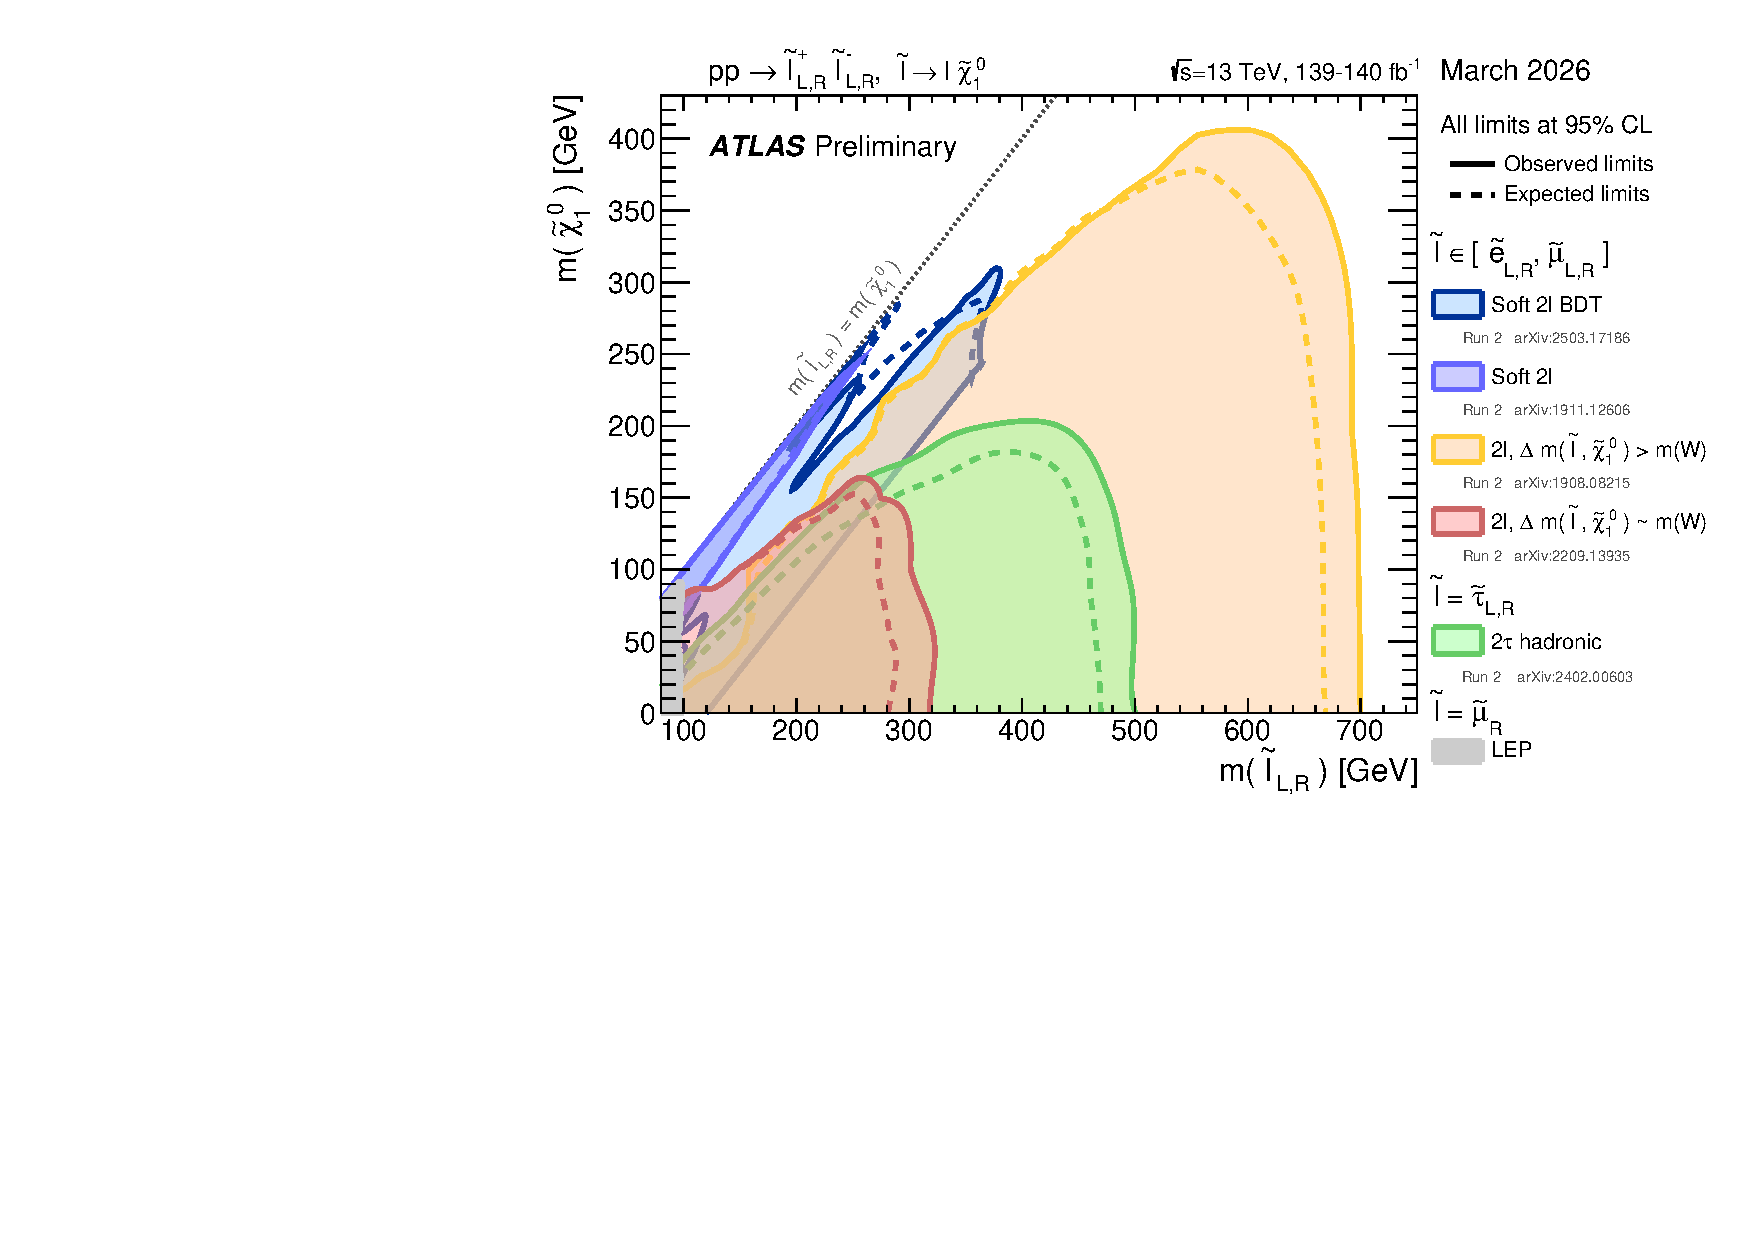
\includegraphics[width=0.8\linewidth]{Figures/slepton_exclusion_2026.pdf}
    \caption{Excluded areas at \qty{95}{\percent} confidence level in the slepton--lightest neutralino mass plane. The figure is retrieved from Ref.~\cite{ATLAS:2026hws}.}
    \label{fig:exclusion}
\end{figure}




%%%%%%%%%%%%%%%%%%%%%
%%% Feynman rules %%%
%%%%%%%%%%%%%%%%%%%%%
\subsection{Feynman Rules for Sleptons}\label{sec:feynman_rules}

In \cref{ch:parton_level} we will calculate \gls{qed} corrections to the parton-level cross section for $q\widebar{q}\to\slepton^*\slepton+X$. To do this, we will need the Feynman rules for interactions between sleptons and electroweak gauge bosons, which we derive in this section.
We will do this by locating the relevant terms in the superlagrangian, integrating over the Grassmann coordinates, and reading off the vertex rules.
To read off an interaction vertex from a Lagrangian, we first extract the numerical factors (not including fields), multiply by symmetry factors, rewrite derivatives as $\partial^\mu\to-ip^\mu$, and multiply the term by $i$. With this convention for the derivatives, all momenta are considered to point \emph{into} the vertex.
As an example, consider an interaction between two scalar fields $\phi$ and $\chi$, described by the Lagrangian term $\mathcal{L} \supset \lambda \phi\phi\partial_\mu\chi$. Its Feynman rule would be written
\begin{equation}
    \inputtikz[baseline=(v.base)]{rules/example_rule} = i \times (2!) \times (-ip^\mu)\lambda = 2\lambda p^\mu,
\end{equation}
where $2!$ is the symmetry factor.

\subsubsection{Electroweak Mixing}
Since the Feynman rules to be derived involve electroweak gauge bosons, we briefly review their properties here.
$W^3_\mu$ and $B_\mu$ mix to give the mass eigenstates $Z_\mu$ (the massive Z boson) and $A_\mu$ (the massless photon), while $W^1_\mu$ and $W^2_\mu$ mix to give the charged W-bosons $W^\pm_\mu$. These mixings are given by
\begin{subequations}
    \begin{align}
        Z_\mu &= c_W W^3_\mu - s_W B_\mu, \label{eq:ew_Z}
        \\
        A_\mu &= c_W B_\mu + s_W W^3_\mu, \label{eq:ew_A}
        \\
        W^\pm_\mu &= \frac{1}{\sqrt{2}} \bigl( W^1_\mu \mp iW^2_\mu \bigr) \label{eq:ew_W},
    \end{align}
\end{subequations}
where $c_W \equiv \cos\theta_W$ and $s_W \equiv \sin\theta_W$, and $\theta_W$ is the Weinberg angle.
The electric charge is related to the weak charge $g$ and hypercharge $g'$ by
\begin{equation}
    e = \frac{gg'}{\sqrt{g^2+g'^2}} = gs_W = g'c_W.
\end{equation}
Some useful relations that follow directly from these definitions are
\begin{subequations}
    \begin{gather}
        W^{1\mu}W^1_\mu + W^{2\mu}W^2_\mu = 2W^{+\mu}W^-_\mu, \label{eq:W12_squared}
        \\
        Z_\mu = \frac{1}{\sqrt{g^2+g'^2}} \bigl( gW^3_\mu - g'B_\mu \bigr),
        \\
        A_\mu = \frac{1}{\sqrt{g^2+g'^2}} \bigl( g'W^3_\mu + gB_\mu \bigr).
    \end{gather}
\end{subequations}

As discussed in \cref{sec:slepton_masses}, the left- and right-handed sleptons $\slepton_{iL/R}$ also mix to form mass eigenstates $\slepton_{i1/2}$.
The sneutrinos, having no right-handed counterpart, do not mix.
The mass mixing matrix $L^i_{\alpha A}$, which we defined in \cref{eq:slepton_mass_mixing}, is unitary, and it follows that
\begin{align*}
    L^{i*}_{LA}L^i_{LB} + L^{i*}_{RA}L^i_{RB}
    &= \delta_{AB},
\end{align*}
i.e.\ $\tilde\ell_{iL}^*\tilde\ell_{iL}+\tilde\ell_{iR}^*\tilde\ell_{iR} = \delta_{AB}\tilde\ell_{iA}\tilde\ell_{iB}$.
Following~\cite{Richardson:2000nt} we define the following slepton couplings
\begin{subequations}
\begin{align}
    \zliab &= \frac{1}{2}\bigl( L^{i*}_{LA}L^i_{LB} - 2s_W^2 \delta_{AB} \bigr),
    \label{eq:zliab}
    \\
    \znuiab &= -\frac{1}{2}\delta_{A=1,B=1},
    \label{eq:znuiab}
\end{align}
\end{subequations}
which will turn out to be useful.


\subsubsection{General Scalar--Vector Component Interactions from Superfields}
We want to find the interaction between sleptons (the scalar component fields of the scalar superfields) and the electroweak gauge bosons (the vector component fields in the vector superfields), thus for our discussion most components in the superfields are irrelevant.
Considering the general superfields in \cref{eq:superfields} the relevant terms remaining are\footnote{
    Note that we only include terms from $\Phi$ with at most one $\theta$ and one $\bar\theta$ since any other term will give zero when multiplied with the vector superfield.
}
\begin{align*}
    \Phi &\supset A + i\theta\sigma^\mu\bar\theta \partial_\mu A,
    \\
    \Phi^\dagger &\supset A^* - i\theta\sigma^\mu\bar\theta \partial_\mu A^*,
    \\
    V &\supset \theta\sigma^\mu\bar\theta V_\mu.
\end{align*}
As can be seen from the general superlagrangian in \cref{eq:general_superlagrangian}, any slepton--gauge boson interaction term must come from the K\"ahler potential---it is the only term containing both scalar and vector superfields. As a reminder, it is given in its general form as
\begin{equation}\label{eq:kahler}
    K[\Phi,\Phi^\dagger,V] = \Phi^\dagger e^{-2qV^aT^a} \Phi.
\end{equation}

When Taylor expanding the exponential in \cref{eq:kahler} only the terms up to quadratic order survives since, in the Wess-Zumino gauge, we have that $V^3=0$.
Using indices $i,j,k$ and $\ell$ to denote different superfields we see that there are two types of interaction terms that can appear in the K\"ahler potential: three-point interactions, given by
\begin{align}
    V_i\Phi_j^\dagger\Phi_k &\supset \theta\sigma^\mu\bar\theta V_{i\mu}
    \Bigl[ A_j^* - i\theta\sigma^\nu\bar\theta\partial_\nu A_j^* \Bigr]
    \Bigl[ A_k + i\theta\sigma^\rho\bar\theta\partial_\rho A_k \Bigr]
    \nonumber
    \\
    \underset{\thetafour}&{\supset} \frac{i}{2} \thetafour \, V_i^\mu \Bigl( A_j^*\lrpartial{\mu} A_k \Bigr), \label{eq:general_three_point}
\end{align}
with $g \lrpartial{\mu} f \equiv g (\partial_\mu f) - (\partial_\mu g)f$;
and four-point interactions, given by
\begin{align}
    V_iV_j\Phi_k^\dagger\Phi_\ell &\supset (\theta\sigma^\mu\bar\theta)V_{i\mu}
    (\theta\sigma^\nu\bar\theta)V_{j\nu}
    A_k^*A_\ell \nonumber
    \\
    &= \frac{1}{2}\thetafour \, V_i^\mu V_{j\mu} A_k^*A_\ell, \label{eq:general_four_point}
\end{align}
where we have used the identity
\begin{equation}\label{eq:theta_sigma_identity}
    (\theta\sigma^\mu\thetabar)(\theta\sigma^\nu\thetabar) = \frac{1}{2}g^{\mu\nu}(\thetatwo)(\thetabartwo).
\end{equation}
This identity is proven in \cref{app:weyl_proof}.
\Cref{eq:general_three_point,eq:general_four_point} will be utilized frequently throughout the following discussion.


\subsubsection{Feynman Rules for Slepton--Gauge Boson Interactions}
Using that the generators of $SU(2)_L$ are $\frac{1}{2}\sigma^a$,
and that $L_i$ and $\bar E_i$ have hypercharges $Y=-1$ and $Y=2$, respectively (see \cref{tab:mssm_fields}),
it is fairly straightforward to write down the relevant terms in the MSSM K\"ahler potential using \cref{eq:kahler}:
\begin{equation*}
    \tilde{\mathcal{L}} \supset L_i^\dagger e^{-g \sigma_a W^a + g'B} L_i + \bar{E}_i^\dagger e^{-2g'B} \bar{E}_i.
\end{equation*}
Expanding the exponential and ignoring the kinetic terms gives
\begin{equation}
    \tilde{\mathcal{L}} \supset
    \underbrace{-2g'B \bar{E}_i^\dagger \bar{E}_i}_{\equiv \tilde{\mathcal{L}}_{3R}}
    + \underbrace{L_i^\dagger (-g\sigma_a W^a + g'B) L_i}_{\equiv \tilde{\mathcal{L}}_{3L}}
    + \underbrace{2g'^2 BB \bar{E}_i^\dagger \bar{E}_i}_{\equiv \tilde{\mathcal{L}}_{4R}}
    + \underbrace{\frac{1}{2} L_i^\dagger (g\sigma_a W^a - g'B)^2 L_i}_{\equiv \tilde{\mathcal{L}}_{4L}}.
    \label{eq:slepton_kahler}
\end{equation}


\paragraph{Three-Point Interactions}\label{sec:three_point}
The three-point interactions come from $\tilde{\mathcal L}_{3R}$ and $\tilde{\mathcal L}_{3L}$ in the first line of \cref{eq:slepton_kahler}. To find them in terms of component fields we expand $\tilde{\mathcal L}_{3L}$:
\begin{equation}
    \tilde{\mathcal{L}}_{3L} =
    -g (W^1-iW^2)\nu_i^\dagger\ell_i - g(W^1+iW^2)\ell_i^\dagger\nu_i
    + (g'B-gW^3)\nu_i^\dagger \nu_i
    + (g'B+gW^3)\ell_i^\dagger\ell_i.
    \label{eq:lagrange_3L}
\end{equation}
All the interactions in terms of component fields can then be found using \cref{eq:general_three_point} and integrating over the Grassmann coordinates.

Three-point interactions involving two charged sleptons come from $\tilde{\mathcal{L}}_{3R}$ and the last term of $\tilde{\mathcal{L}}_{3L}$ in \cref{eq:lagrange_3L}:
\begin{align*}
    \mathcal{L}_{V\tilde\ell\tilde\ell} &= -ig' B^\mu \Bigl( \tilde{\ell}_{iR} \lrpartial{\mu} \tilde{\ell}_{iR}^* \Bigr)
    +\frac{i}{2} (gW^{3\mu}+g'B^\mu) \Bigl( \tilde{\ell}_{iL}^* \lrpartial{\mu} \tilde{\ell}_{iL} \Bigr)
    \\
    &= ie \biggl( A^\mu - \frac{s_W^2}{s_Wc_W}Z^\mu \biggr) \Bigl( \tilde{\ell}_{iR}^* \lrpartial{\mu} \tilde{\ell}_{iR} \Bigr)
    % \\ &\quad
    + \biggl[ ie A^\mu + \frac{ie}{2s_Wc_W} (1-2s_W^2) Z^\mu \biggr] \Bigl( \tilde{\ell}_{iL}^* \lrpartial{\mu}  \tilde{\ell}_{iL} \Bigr),
\end{align*}
which can be rewritten in terms of the sleptons' mass eigenstates, giving
\begin{align}
    \mathcal{L}_{V\tilde\ell\tilde\ell}
    &= \biggl[ ieA^\mu \delta^{AB} + \frac{ie}{s_Wc_W} \zliab Z^\mu \biggr] \tilde{\ell}_{iA}^* \lrpartial{\mu} \tilde{\ell}_{iB},
    \label{eq:L_Vll}
\end{align}
where $A$ and $B$ label the sleptons' mass eigenstates.

Three-point interactions involving two sneutrinos come from the third term of $\tilde{\mathcal{L}}_{3L}$ in \cref{eq:lagrange_3L}:
\begin{align}
    \mathcal{L}_{V\tilde\nu\tilde\nu} &= \frac{i}{2} (g'B_\mu-gW^3_\mu) \Bigl( \tilde\nu_{iL}^* \lrpartialUpper{\mu} \tilde\nu_{iL} \Bigr)
    \nonumber
    \\
    &= \frac{ie}{s_Wc_W} \znuiab Z_\mu \Bigl( \tilde\nu_{iA}^* \lrpartialUpper{\mu} \tilde\nu_{iB} \Bigr).
    \label{eq:L_Vnunu}
\end{align}
The remaining terms, the first two terms of $\tilde{\mathcal{L}}_{3L}$ in \cref{eq:lagrange_3L}, give the three-point interactions involving both a charged slepton and a sneutrino. The Lagrangian terms are
\begin{align}
    \mathcal{L}_{V\tilde\ell\tilde\nu} &= -\frac{ig}{2} \biggl[
        (W^1_\mu-iW^2_\mu) \Bigl( \tilde\nu_{iL}^* \lrpartialUpper{\mu} \tilde\ell_{iL} \Bigr)
        + (W^1_\mu + iW^2_\mu) \Bigl( \tilde\ell_{iL}^* \lrpartialUpper{\mu} \tilde\nu_{iL} \Bigr)
    \biggr]
    \nonumber
    \\
    &= -\frac{ie}{\sqrt{2}s_W} \biggl[
        W^+_\mu \Bigl( \tilde\nu_{iL}^* \lrpartialUpper{\mu} \tilde\ell_{iL} \Bigr)
        + W^-_\mu \Bigl( \tilde\ell_{iL}^* \lrpartialUpper{\mu} \tilde\nu_{iL} \Bigr)
    \biggr].
    \label{eq:L_Vlnu}
\end{align}

The resulting Feynman rules from the Lagrangian terms in \cref{eq:L_Vll,eq:L_Vlnu,eq:L_Vnunu} are given in \cref{tab:slepton_rules}.
We can see that they coincide perfectly with Refs.~\cite{Richardson:2000nt,Rosiek:1989sce}.

\paragraph{Four-Point Interactions}
The four-point interactions come from $\tilde{\mathcal L}_{4R}$ and $\tilde{\mathcal L}_{4L}$ in the second line of \cref{eq:slepton_kahler}.
Using the anticommutator relation for Pauli matrices:
$\{\sigma_a,\sigma_b\} = 2 \delta_{ab}$,
it is easy to show that
$(\sigma_a W^a)^2 = W_aW^a$.
Using this we can expand $\tilde{\mathcal{L}}_{4L}$ to get\footnote{
    Here we place the indices of $W$ downstairs, reserving the superscripts for exponents.
}
\begin{equation}
    \begin{split}
        \tilde{\mathcal{L}}_{4L} &=
        \frac{1}{2} \Bigl[
            g^2 (W_1^2+W_2^2) + (gW_3+g'B)^2
        \Bigr] \ell_i^\dagger \ell_i
        \\ &\quad
        + \frac{1}{2} \Bigl[
            g^2 (W_1^2+W_2^2) + (gW_3 - g'B)^2
        \Bigr] \nu_i^\dagger \nu_i
        \\ &\quad
        -gg'B \Bigl[
            (W_1-iW_2)\nu_i^\dagger\ell_i + (W_1+iW_2)\ell_i^\dagger\nu_i
        \Bigr].
        \label{eq:lagrange_4L}
    \end{split}
\end{equation}
The interaction terms can then be found by applying \cref{eq:general_four_point} and integrating over the Grassmann coordinates.

Four-point interactions involving two charged sleptons come from $\tilde{\mathcal{L}}_{4R}$ and the first term of $\tilde{\mathcal{L}}_{4L}$ in \cref{eq:lagrange_4L}:
\begin{align*}
    \mathcal{L}_{VV\tilde\ell\tilde\ell}
    &= \frac{1}{4} \Biggl[
        \frac{2e^2}{s_W^2} W^{+\mu}W^-_\mu + 4e^2 A^\mu A_\mu
        + \frac{4e^2}{s_Wc_W}(1-2s_W^2) A^\mu Z_\mu
        \\ &\quad
        + \frac{e^2}{s_W^2c_W^2}(1 - 2s_W^2)^2 Z^\mu Z_\mu
    \Biggr] \tilde\ell_{iL}^*\tilde\ell_{iL}
    + e^2 \biggl( A^\mu A_\mu - \frac{2s_W}{c_W} A^\mu Z_\mu + \frac{s_W^2}{c_W^2} Z^\mu Z_\mu \biggr)
    \tilde\ell_{iR}^*\tilde\ell_{iR},
\end{align*}
which in terms of mass eigenstates is
\begin{equation}
    \begin{split}
        \mathcal{L}_{VV\tilde\ell\tilde\ell}
        &= \tilde\ell_{iA}^*\tilde\ell_{iB} \Biggl[
            \frac{e^2}{2s_W^2} W^{+\mu}W^-_\mu L^{i*}_{LA}L^i_{LB}
            + e^2 \delta^{AB} A^\mu A_\mu
            \\ & \quad
            + \frac{2e^2}{s_Wc_W} \zliab A^\mu Z_\mu
            + \frac{e^2}{c_W^2} \Biggl(
                \frac{1-4s_W^2}{4s_W^2} L_{LA}^{i*}L_{LB}^i + s_W^2 \delta^{AB}
            \Biggr) Z^\mu Z_\mu
        \Biggr].
    \end{split}
    \label{eq:L_VVll}
\end{equation}

The terms involving two sneutrinos come from the second line of $\tilde{\mathcal{L}}_{4L}$ in \cref{eq:lagrange_4L}:
\begin{align}
    \hspace{-0.5em} \mathcal{L}_{VV\tilde\nu\tilde\nu}
    &= \frac{1}{4} \Biggl[
        2\frac{e^2}{s_W^2} W^{+\mu}W^-_\mu
        + \frac{e^2}{s_W^2c_W^2} Z^\mu Z_\mu
    \Biggr] \tilde\nu_i^*\tilde\nu_i,
    \label{eq:L_VVnunu}
\end{align}
and the terms involving both a charged slepton and a sneutrino come from the last term of $\tilde{\mathcal{L}}_{4L}$ in \cref{eq:lagrange_4L}:
\begin{equation}
    \hspace{-0.5em} \mathcal{L}_{VV\tilde\ell\tilde\nu}
    = -\frac{e^2}{\sqrt{2}} \biggl(
        \frac{1}{s_W} A^\mu - \frac{1}{c_W} Z^\mu
    \biggr)
    (W^+_\mu \tilde\nu_{iL}^*\tilde\ell_{iL} + W^-_\mu \tilde\ell_{iL}^*\tilde\nu_{iL}).
    \label{eq:L_VVlnu}
\end{equation}

The resulting Feynman rules from the Lagrangian terms in \cref{eq:L_VVll,eq:L_VVlnu,eq:L_VVnunu} are given in \cref{tab:slepton_rules} (note the symmetry factor of $2$ from couplings with $Z^\mu Z_\mu$ and $A^\mu A_\mu$).
They are exactly the same as the ones found in Ref.~\cite{Rosiek:1989sce}\footnote{
    We are not able to cross-check these rules with Richardson's thesis~\cite{Richardson:2000nt} as he does not include four-point interactions.
}

\subsubsection{Summary}
We have derived the Feynman rules for slepton--gauge boson interactions that are necessary for the calculation of \gls{qed} corrections to slepton pair production in \cref{ch:parton_level}. The full set of derived Feynman rules are shown in \cref{tab:slepton_rules}.
In addition to sleptons, we will also make use of the electroweak interactions of quarks.
For completeness, these are also included in \cref{tab:slepton_rules}, and are taken from \cite{Richardson:2000nt}.
Their Feynman rules make use of the couplings $Z_{q_L}$ and $Z_{q_R}$, given by
\begin{align}
    Z_{q_L} &= \frac{1}{2}\Bigl( Q_q s_W^2 - T^3_{q_L} \Bigr),\\
    % Z_{u_L} &= -\frac{1}{4}(1 - 2Q_u s_W^2) \\
    % Z_{d_L} &= \frac{1}{4}(1 + 2Q_d s_W^2) \\
    Z_{q_R} &= \frac{1}{2}Q_q s_W^2,
\end{align}
where $Q_q$ is the electric charge of quark $q$, and we remind the reader that the weak isospin is $T^3 = \pm\frac{1}{2}$ for up- and down-type quarks, respectively.

Propagators are given by (using the Feynman gauge for vector bosons)~\cite{Peskin:1995ev}
\begin{equation}\label{eq:propagators_and_externals}
\begin{split}
    \inputtikz[baseline=(a.base)]{propagators/prop_fermion} &= \frac{i(\slashed{p}+m)}{p^2-m^2+i\epsilon},
    \\
    \inputtikz[baseline=(a.base)]{propagators/prop_boson} &= \frac{-ig_{\mu\nu}}{p^2-m^2+i\epsilon},
    \\
    \inputtikz[baseline=(a.base)]{propagators/prop_scalar} &= \frac{i}{p^2-m^2+i\epsilon}.
\end{split}
\end{equation}
External lines in Feynman diagram contribute a factor of unity for (charged) scalars, while incoming/outgoing fermions, anti-fermions and vector bosons contribute spinors $u(p)$/$\widebar{u}(p)$, $\widebar{v}(p)$/$v(p)$ and polarization vectors $\eps_\mu(p)$/$\eps_\mu^*(p)$, respectively.
% External lines in Feynman diagram contribute a factor of unity for (charged) scalars, while incoming (outgoing) fermions, anti-fermions and vector bosons contribute spinors $u(p)$ ($\widebar{u}(p)$), $\widebar{v}(p)$ ($v(p)$) and polarization vectors $\eps_\mu(p)$ ($\eps_\mu^*(p)$), respectively.
% External lines in Feynman diagram contribute a factor of unity for (charged) scalars, while incoming (outgoing) fermions, anti-fermions and vector bosons contribute spinors $u$ ($\widebar{u}$), $\widebar{v}$ ($v$) and polarization vectors $\eps_\mu$ ($\eps_\mu^*$), respectively.
% polarization vectors $\eps_\mu(p)$ ($\eps_\mu^*(p)$) for incoming (outgoing) vector bosons, and spinors $u(p)$ ($\widebar{u}(p)$) and $\widebar{v}(p)$ ($v(p)$) for incoming (outgoing) fermions and anti-fermions, respectively.


\begin{table}[ht]
    \centering
    \caption{The Feynman rules for electroweak slepton--gauge boson interactions derived in \cref{sec:feynman_rules}, and the corresponding electroweak interactions of the Standard Model quarks~\cite{Richardson:2000nt}. $V^{1,2}_\mu$ and $s_{1,2}$ denote general vectors and charged scalars, $q$ and $\widebar{q}$ denote (same-flavor) quarks and anti-quarks, while $u_i$ and $d_i$ denote the $i$'th generation of up- and down-type quarks, respectively.}
    % We also include the electroweak interactions of Standard Model quarks~\cite{Richardson:2000nt}, as these are relevant for calculations in \cref{ch:parton_level}. Here $q$ and $\widebar{q}$ denote general quarks and anti-quarks, while $u_i$ and $d_i$ denote $i$'th generation of up- and down-type quarks, respectively.}
    \label{tab:slepton_rules}
    \renewcommand{\arraystretch}{1.8}
    \begin{tabular}{|c|c|c|}
        \hline
        \multicolumn{3}{|c|}{\textbf{Three-point interactions}}
        \\ \hline
        Coupling & Feynman rule & Diagram
        \\ \hline
        $\gamma\tilde\ell_{iA}^*\tilde\ell_{iB}$ & $ie (p+p')^\mu \delta^{AB}$ & \multirow{5}{*}{\inputtikz[baseline=(v)]{rules/general-3point}}
        \\
        $Z\tilde\ell_{iA}^*\tilde\ell_{iB}$ & $\frac{ie}{s_Wc_W} \zliab (p+p')^\mu$ &
        \\
        $Z\tilde\nu_{iA}^*\tilde\nu_{iB}$ & $\frac{ie}{s_Wc_W} \znuiab (p+p')^\mu$ &
        \\
        $W^-\tilde\ell_{iA}^*\tilde\nu_{iL}$ & $-\frac{ie}{\sqrt{2} s_W} L^{i*}_{LA} (p+p')^\mu$ &
        \\
        $W^+\tilde\nu_{iL}^*\tilde\ell_{iA}$ & $-\frac{ie}{\sqrt{2} s_W} L^i_{LA} (p+p')^\mu$ &
        \\ \hline\hline
        \multicolumn{3}{|c|}{\textbf{Four-point interactions}}
        \\ \hline
        Coupling & Feynman rule & Diagram
        \\ \hline
        $\gamma\gamma \tilde\ell_{iA}^*\tilde\ell_{iB}$ & $2ie^2\delta^{AB}g^{\mu\nu}$ & \multirow{10}{*}{\inputtikz[baseline=(v)]{rules/general-4point}}
        \\
        $\gamma Z \tilde\ell_{iA}^*\tilde\ell_{iB}$ & $\frac{2ie^2}{s_Wc_W} \zliab g^{\mu\nu}$ &
        \\
        $Z Z \tilde\ell_{iA}^*\tilde\ell_{iB}$ & $\frac{2ie^2}{c_W^2} \Bigl( \frac{1-4s_W^2}{4s_W^2} L_{LA}^{i*}L_{LB}^i + s_W^2 \delta^{AB} \Bigr) g^{\mu\nu}$ &
        \\
        $W^+ W^- \tilde\ell_{iA}^*\tilde\ell_{iB}$ & $\frac{ie^2}{2s_W^2} L^{i*}_{LA} L^i_{LB} g^{\mu\nu}$ &
        \\
        $W^+ W^- \tilde\nu_{iL}^*\tilde\nu_{iL}$ & $\frac{ie^2}{2s_W^2} g^{\mu\nu}$ &
        \\
        $Z Z \tilde\nu_{iL}^*\tilde\nu_{iL}$ & $\frac{ie^2}{2s_W^2c_W^2} g^{\mu\nu}$ &
        \\
        $\gamma W^- \tilde\ell_{iA}^*\tilde\nu_{iL}$ & $-\frac{ie^2}{\sqrt{2}s_W} L^{i*}_{LA} g^{\mu\nu}$ &
        \\
        $\gamma W^+ \tilde\nu_{iL}^*\tilde\ell_{iA}$ & $-\frac{ie^2}{\sqrt{2}s_W} L^i_{LA} g^{\mu\nu}$ &
        \\
        $Z W^- \tilde\ell_{iA}^*\tilde\nu_{iL}$ & $\frac{ie^2}{\sqrt{2}c_W} L^{i*}_{LA} g^{\mu\nu}$ &
        \\
        $Z W^+ \tilde\nu_{iL}^*\tilde\ell_{iA}$ & $\frac{ie^2}{\sqrt{2}c_W} L^i_{LA} g^{\mu\nu}$ &
        \\ \hline\hline
        \multicolumn{3}{|c|}{\textbf{SM interactions}}
        \\ \hline
        Coupling & Feynman rule & Diagram
        \\ \hline
        $q\widebar{q}\gamma$ & $-ieQ_q\gamma^\mu$ & \multirow{3}{*}{\inputtikz[baseline=(v)]{rules/general_sm}}
        \\
        $q\widebar{q}Z$ & $\frac{ie}{s_Wc_W}\gamma^\mu\Bigl[Z_{q_L}(1-\gamma^5)+Z_{q_R}(1+\gamma^5)\Bigr]$ &
        \\
        $d_i\widebar{u}_i W^-$ & $\frac{-ie}{2\sqrt{2}\,s_W}\gamma^\mu(1-\gamma^5)$ &
        \\ \hline
    \end{tabular}
\end{table}
